\documentclass[a4paper,12pt]{book}
\usepackage{graphicx}
\usepackage[export]{adjustbox}
\usepackage{subcaption}
\graphicspath{{Pics/}}
\usepackage{charter}
\usepackage{fancyhdr}
\usepackage{enumerate}
\usepackage{enumitem}
\usepackage{siunitx}
\usepackage{amssymb}
\usepackage{longtable}
\usepackage{multicol}
\usepackage{multirow}
\usepackage{hhline}
\usepackage{parskip}
\setlength{\parskip}{6pt}
\usepackage{ragged2e}
\usepackage{geometry} %margin
\geometry{left=2.1cm,right=2.1cm,top=3cm,bottom=3cm}
\usepackage{setspace}
\SetSinglespace{1.2}
\singlespacing
\renewcommand{\ttfamily}{\fontfamily{pcr}\selectfont}
%\renewcommand{\familydefault}{\rmdefault}

\usepackage[,table]{xcolor}
\definecolor{LightBlue}{cmyk}{0.16,0.03,0.04,0}
\definecolor{Title}{cmyk}{0.8,0.1,0,0.3}
\setlength{\arrayrulewidth}{0.3mm}
\setlength{\tabcolsep}{2pt}
\setlength{\headheight}{15pt}
\renewcommand{\arraystretch}{1}
\usepackage{tikz}
\usepackage{nicematrix}
\newcommand*\circled[1]{\tikz[baseline=(char.base)]{\node[shape=circle,draw,inner sep=1pt] (char) {#1};}}

\newcolumntype{s}{>{\columncolor{Title}\RaggedLeft} m{3.5em}} % columntype for chapter title
\newcolumntype{d}{>{\columncolor{LightBlue}\RaggedRight} m{\textwidth}} % columntype for code bloc
\newcolumntype{a}{>{\columncolor{LightBlue}\RaggedRight} m{0.96\textwidth}} % columntype for secondary code bloc

\usepackage{titlesec}
\usepackage[hidelinks]{hyperref}
\urlstyle{same}

\captionsetup[figure]{labelsep=period,font={bf}}
\captionsetup[table]{font={bf},labelsep=period}

\newcommand{\titlename}{}

\newcommand{\chaptertitle}[2]{ %reset chapter format
\vspace{-120pt}
\gdef\titlename{#1}
{
\SetSinglespace{1.1}
\singlespacing
\Huge\bfseries
\setlength{\tabcolsep}{8pt}
\renewcommand{\arraystretch}{1.5}
\begin{tabular}{s >{\RaggedRight}m{14.5em}}
\textcolor{white}{Chapter\newline\thechapter}&\textcolor{Title}{#2}
\end{tabular}
}
}

\newcommand{\partpic}[1]{%insert picture
    \tikz[remember picture,overlay] \node at (current page.center){\includegraphics[width=\paperwidth]{#1}};
}

\titleformat{\part} %reset part %format
{\huge\bfseries} % format
{} % label
{0em} % sep
{\Centering} % before-code

\titleformat{\chapter} %reset chapter %format
{\huge\bfseries} % format
{} % label
{0em} % sep
{\Centering} % before-code
\titlespacing{\chapter}{0pt}{0pt}{0pt}

\titleformat{\section} %reset section %format
{\Large\bfseries} % format
{\textcolor{Title}{\thesection}} % label
{0.5em} % sep
{\color{Title}} % before-code
\titlespacing{\section}{0pt}{12pt}{6pt}

\titleformat{\subsection} %reset subsection %format
{\large\bfseries} % format
{\textcolor{Title}{\thesubsection}} % label
{0.5em} % sep
{\color{Title}} % before-code
\titlespacing{\subsection}{0pt}{8pt}{6pt}

\newenvironment{term}[1]{
    \textbf{#1}

    \leftskip 1em
    \parskip 0pt
}

\newenvironment{secterm}[1]{
    \textbf{#1}

    \leftskip 2em
    \parskip 0pt
}

\newenvironment{codebloc}{ %define code bloc style
    \ttfamily\footnotesize
    \renewcommand{\arraystretch}{1}
}

\newcommand{\note}[2][NOTE]{ %Note/Tips
\vspace{6pt}
\begin{tabular}{b{\textwidth}}
\hline
\fontfamily{phv}\selectfont \textbf{#1}\\
\leftskip 1em #2\\
\hline
\end{tabular}
}

\newcommand{\secnote}[2][NOTE]{ %Note/Tips
\vspace{6pt}
\begin{tabular}{b{0.93\textwidth}}
\hline
\fontfamily{phv}\selectfont \textbf{#1}\\
\leftskip 1em #2\\
\hline
\end{tabular}
}

\title{ESP32-C3 Wireless Adventure\par \Large A comprehensive guide to IoT}
\author{Espressif Systems}
\date{\today}

\pagestyle{fancy} % reset head&foot
\fancyhead{} % clear all header fields
\renewcommand\headrulewidth{0pt}
\fancyfoot{} % clear all footer fields
\setcounter{chapter}{7}

\begin{document}

\fancyfoot[LE]{\fontfamily{cmss}\selectfont{\textbf{\thepage} \ \textit{ESP32-C3 Wireless Adventure: A comprehensive guide to IoT}}}
\fancyfoot[RO]{\fontfamily{cmss}\selectfont{\textit{Chapter \thechapter. \titlename} \ \textbf{\thepage}}}

\chapter[Local Control]{\chaptertitle{Local Control}{Local Control}}

\vspace{36pt}
In Chapter 7, we learnt about basics of Wi-Fi and Bluetooth, as well as several common network configuration methods. Through the introduction and practice in Chapter 7, you should be able to configure devices and connect them to Wi-Fi routers. On this basis, this chapter will introduce how to implement local control of devices based on Wi-Fi and Bluetooth, and realize local control with ESP32-C3. It is intended to explain the definition and process of local control, along with some common local control communication protocols, and help you to build your own local control framework for smart lights based on ESP32-C3.

\section{Introduction to Local Control}
This section first introduces what local control is and its usage conditions, scenarios, and advantages. Then it will expound on the device discovery function and data communication protocols involved in local control, and how to choose the data transmission medium for local control. After reading this section, you will have a full understanding of local control of devices.

As the name suggests, local control refers to operating controlled devices within a certain distance through a series of methods such as hardware switches, touch buttons, infrared remote control, smartphones, and computer networks. It is ubiquitous in our daily life, such as setting air conditioners through infrared remote controls, controlling voice-activated equipment through voice commands, and turning on household lighting through switches or smartphone apps. The concept and technology of local control have become deeply integrated into every aspect of our daily lives.

You may have noticed that some of the examples listed above are performed through hardware circuit switches or wireless communication technologies such as infrared remote control, while others involve voice recognition, and data communication technologies such as the Internet of Things. In this book, we will focuse on the data communication technology of IoT, and help you build your own local control framework to control the ESP32-C3 smart lights.

Within the Internet of Things, each device needs to transmit commands through certain data communication method. Some common ways are as follows:

\begin{itemize}[leftmargin=1.5em]
    \item \textbf{Using Wi-Fi or Ethernet}. Generally, devices based on Wi-Fi and Ethernet natively run the TCP/IP protocol stack, which greatly reduces the workload of protocol adaptation and development. When performing local communication, they also need a gateway or Wi-Fi router.
    \item \textbf{Using short-range wireless communication technologies} such as Bluetooth and ZigBee, which is suitable for data transmission between low-speed and low-power devices.
\end{itemize}

According to the functional characteristics of ESP32-C3, we will introduce two commonly used local control technologies in this chapter, namely through Wi-Fi or Bluetooth within a LAN.

The network topology centered on Wi-Fi is shown in Figure 8.1. The command sending devices (smartphone or PC) should be in the same LAN as the controlled device, and send data to the device through Wi-Fi. But for Bluetooth control, there is no need of Wi-Fi routers, as data can be directly transmitted between the smartphone and the controlled device via Bluetooth.

\begin{figure}[!h]
    \centering
    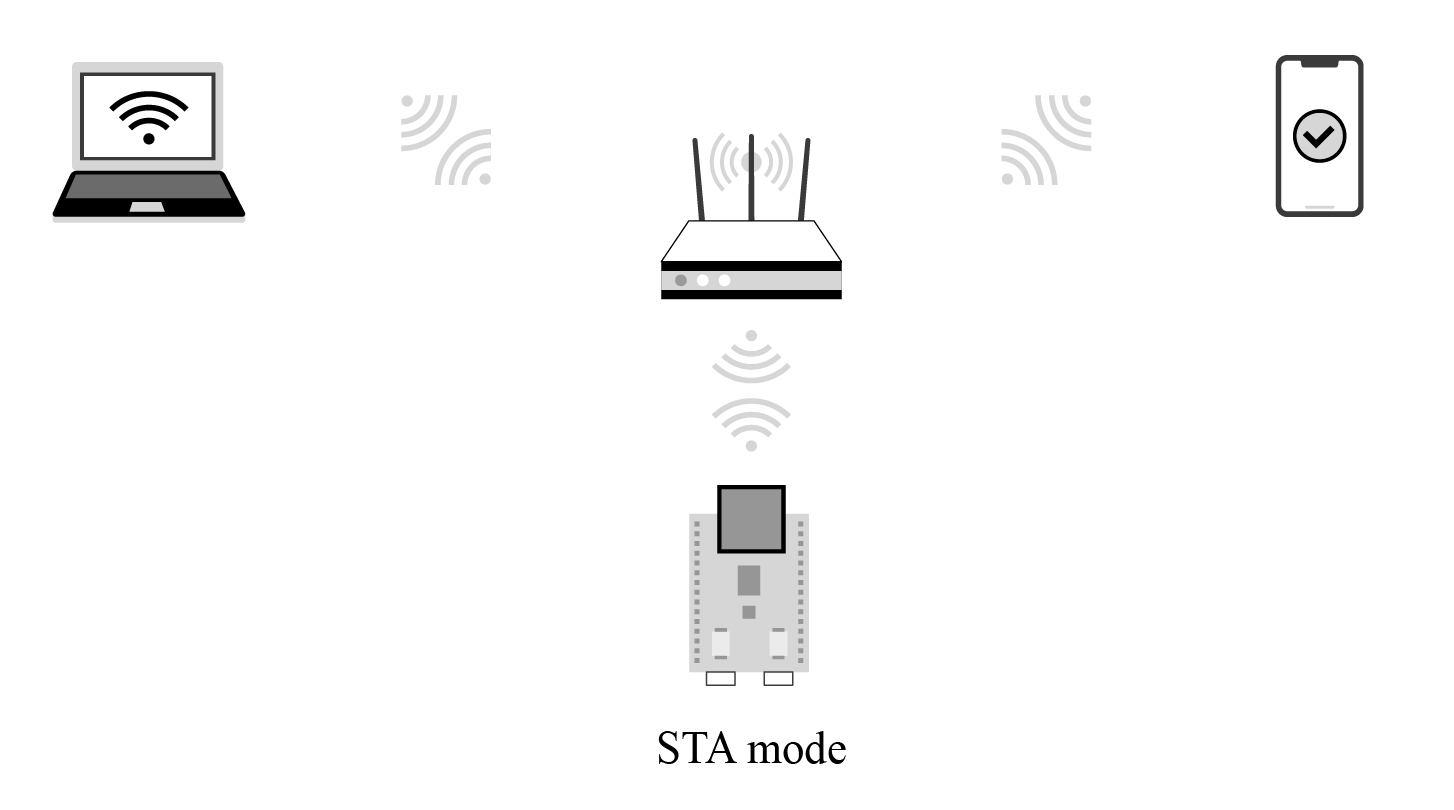
\includegraphics[width=0.6\textwidth]{D8Z/8-1}
    \caption{Network topology centered on Wi-Fi within a LAN}
\end{figure}

Using Bluetooth is simpler than using Wi-Fi as Bluetooth does not require Wi-Fi routers. However, in practice, if the IoT device wants to access cloud platforms, it needs Wi-Fi routers to connect to the Internet and then the cloud platform. Moreover, smartphones are mostly connected to Wi-Fi routers. Therefore, an LAN usually includes Wi-Fi routers, which makes it convenient to use Wi-Fi for local control. If the IoT device does not need access to cloud platforms, Bluetooth can be a good option for local control. You can select one of the methods according to whether your device needs access to cloud platforms.

\begin{itemize}[leftmargin=1.5em]
    \item If \textbf{yes}, it is recommended to choose Wi-Fi, as it supports multiple smartphones controlling one device at the same time, and its transmission bandwidth is larger than that of Bluetooth. You can use Bluetooth only for network configuration, and then stop its protocol stack to save ESP32-C3’s resources.
    \item If \textbf{no}, you can use Bluetooth instead of Wi-Fi to exchange data between the smartphone and controlled device.
\end{itemize}

\subsection{Application of Local Control}
Most IoT devices are connected to cloud platforms which forward commands from smartphones to implement remote control. Such control depends on the Internet provided by Wi-Fi routers to maintain the link between the controlled device and cloud platforms. But once the Wi-Fi routers disconnect from the Internet, remote control will be paralyzed. At this point, local control will be a good supplement for sending commands, thus preventing the IoT devices from a full-out breakdown due to network exceptions.

As shown in Figure 8.1, a local control framework based on Wi-Fi in a LAN consists of a Wi-Fi router, a controlling device, and a controlled device. The controlling device can be a smartphone or a computer that can run TCP/IP protocol stack. It should be connected to the same Wi-Fi router as the controlled device, to ensure that they are in the same LAN for data communication.

As for local control based on Bluetooth, Wi-Fi routers are not needed. Smartphones can directly connect to the controlled device through Bluetooth and realize point-to-point data transmission.

\subsection{Advantages of Local Control}
Local control only requires data to be transmitted within the LAN instead of through the Internet. Therefore, it functions with shorter delay and faster response. Moreover, as the data only interacts within the LAN composed of the controlled device, a Wi-Fi router and the controlling devices, there is lower probability of data being stolen or modified, hence enhancing data privacy and security.
In addition, local control saves Internet bandwidth. It is not vulnerable to Internet disconnection. As long as the two parties are in the same LAN or linked through Bluetooth, the control can be maintained. For some products without access to cloud platforms, local control is the only means for smartphones to take charge of them.

Considering these advantages, local control is increasingly favored by IoT companies. More and more SDKs and products support local control functions. For example, the ESP RainMaker, a complete IoT platform developed by Espressif, includes a smartphone app to implement local control.

\subsection{Discovering Controlled Devices through Smartphones}
For local control based on Wi-Fi wireless transmission media, data runs on the TCP/IP protocol stack. The following two issues should be solved since the smartphone is not directly connected to the controlled device. How does the smartphone find the controlled device, and how does the smartphone communicate with the controlled device?

How does the smartphone find the controlled device, that is, how does the smartphone know the IP address of the controlled device? Since all data is transmitted based on the IP layer, obtaining the IP address of the controlled device is a prerequisite for subsequent data communication. You may consider: “I can log in to the Wi-Fi router interface and check the IP address of the controlled device directly on the Wi-Fi router interface, right?” Yes, you can certainly obtain the IP address of the controlled device in this way. However, manually querying IP addresses completely goes against the original intention of IoT technology to bring convenience. Thus, a technology is required to automatically discover the controlled device. This part will be discussed in detail in section 8.2.

For the local control frameworks based on Bluetooth control, you can learn from the Bluetooth scanning introduced in Chapter 7 that the Bluetooth of the controlled device will broadcast its own Bluetooth information, and the smartphone only needs to scan the Bluetooth of the controlled device. Discovering the controlled device through Bluetooth is much simpler than Wi-Fi. After the smartphone connects to the Bluetooth of the controlled device, it can send data to the device. In addition, Bluetooth transmission does not depend on the TPC/IP protocol stack, as it has its own transmission protocol. This part will be introduced in detail in section 8.3.

\subsection{Data Communication Between Smartphones and Devices}
How does smartphones communicate with controlled devices?

When using Wi-Fi wireless transmission media, a smartphone can communicate with the controlled device through TCP/IP protocol or UDP protocol after obtaining the IP address of the controlled device. Generally speaking, as the receiver, the controlled device receives control commands sent by the smartphone in local control; and the smartphone,as the sender, sends control commands to the controlled device. Therefore, the controlled device plays the role of a server; and the smartphone plays the role of a client, allowing multiple clients to send control commands to the server. This part will be introduced in detail in section 8.3.

\section{Common Local Discovery Methods}
In section 8.1.4, we mentioned how to discover controlled devices in the LAN using Wi-Fi wireless transmission media. In the TCP/IP protocol stack, discovering the controlled device means obtaining the IP address of the controlled device.

In a LAN, how to obtain the peer’s IP address is a problem worth studying. A common protocol for obtaining the peer’s IP address is the Reverse Address Resolution Protocol (RARP). This protocol sends query packets with knowing the peer’s MAC address, and the gateway server parses its own ARP table to obtain the IP address of the queried MAC device. If you are familiar with LAN, you may immediately associate with the Address Resolution Protocol (ARP), which is a protocol that sends query packets with knowing the peer’s IP address. The peer device or gateway device replies with the MAC address corresponding to the IP address after querying its own ARP table. ARP and RARP are a pair of protocols that mutually resolve network layer addresses and data link layer addresses. However, these two protocols both need to know the peer’s network layer address or data link layer address. This feature brings difficulty to IoT applications as the network layer address and data link layer address of a device in the LAN are difficult to be obtained. Thus, this subsection will introduce the local discovery technology that is truly suitable for IoT.

Local discovery is to discover information about nodes in the LAN, including address information for communication with nodes, application service information supported by nodes, and customised information. For example, mDNS (Multicast DNS, which will be introduced in subsection 8.2.4) is a commonly-used local discovery protocol. The principle of local discovery is to send a message, and the peer will inform the sender of its device information after receiving the message. Now the problem that needs to be solved is how to ensure that the peer can receive the message sent by the sender.

In fact, if you understand the classification of IP addresses, you will know that in addition to the more commonly-used point-to-point communication (unicast), there are also one-to-many (multicast) and one-to-all (broadcast) communications. IP addresses can be divided into unicast addresses, multicast addresses, and broadcast addresses. Unicast needs to know the peer’s IP address, so it is not suitable for local discovery. Multicast and broadcast do not need to know the peer’s IP address. They send messages to specific addresses, and the peer can receive the messages as long as it monitors this address. Thus, multicast and broadcast are suitable for discovering devices in the LAN, and the peer can receive the message sent by the sender with these two technologies.

\subsection{Broadcast}
Broadcast refers to sending messages to all possible receivers in the network. There are two major applications of broadcast:

\begin{itemize}[leftmargin=1.5em,noitemsep]
    \item Locating a host in the local network.
    \item Reducing the packet flow in the local network, so that one message can notify all hosts in the local network.
\end{itemize}

Common broadcast application messages include:

\begin{term}{Address Resolution Protocol (ARP)}
    It can be used to broadcast an ARP request in the local network: “Please tell me what the MAC address of the device with IP address \textit{a.b.c.d} is”. ARP broadcast is MAC broadcast on layer 2 (link layer), not the IP broadcast on layer 3 (network layer).
\end{term}

\begin{term}{Dynamic Host Configuration Protocol (DHCP)}
    If there is a DHCP server on the local network, the DHCP client sends a DHCP request for the destination IP address (usually 255.255.255.255), and the DHCP server on the same network can receive the request and reply with an assigned IP address.
\end{term}

Broadcast mainly uses the UDP protocol (see subsection 8.3.3 for details) instead of the TCP protocol (see subsection 8.3.1 for details) as it is more suitable for unicast.

\subsubsection{1. Broadcast addresses}
Broadcast addresses include MAC broadcast addresses on layer 2 (link layer) (FF:FF:FF:FF:\\FF:FF) and IP broadcast addresses on layer 3 (network layer) (255.255.255.255), hereinafter referred to as layer 2 addresses and layer 3 addresses. This section mainly introduces layer 3 addresses. Generally, when the layer 3 address of a message is all 255, the layer 2 address is usually all FF. This is because a message with a layer 3 address full of 255 means that all devices in the local network will receive this message. If the layer 2 address of the message is not all FF, the message will be discarded during the layer 2 address processing of the receiving device. For the receiving device, if the layer 2 address of the message is not a broadcast address, nor the local MAC address and multicast MAC address (such as 01:00:5E:\textit{XX}:\textit{XX}:\textit{XX}), it will be discarded and not processed. Therefore, generally, if the layer 3 address is a broadcast address, so is the layer 2 address.

IPv4 addresses consist of a subnet ID and a host ID. For example, for a device with an IP address of 192.168.3.4 and a subnet mask of 255.255.255.0, its subnet ID and host ID are calculated from the IP address and subnet mask. In this example, the subnet ID is 192.168.3.0 and the host ID is 4. When the subnet ID and host ID are all 255, it is a broadcast address; it is also a broadcast address when only the host ID is all 255. For example, if you have a subnet of 192.168.1/24, then 192.168.1.255 is the broadcast address of this subnet.

You may wonder, what is the difference between a broadcast address with a subnet ID and host ID of all 255 and a broadcast address with only a host ID of 255?

The broadcast range of the first address is larger than that of a specific subnet. For example, a Wi-Fi router has two subnets, 192.168.1/24 and 192.168.2/24. If a host with IP address of 192.168.1.2 in the subnet 192.168.1/24 sends a message to the destination address 192.168.1.255, the Wi-Fi router will only forward the message to the host in the subnet 192.168.1/24, and will not forward it to the host in the subnet 192.168.2/24. If the host sends a message to the destination address 255.255.255.255, the Wi-Fi router will forward the message to hosts in both subnets. Therefore, the broadcast address with a host ID of 255 is also called a subnet-directed broadcast address. By using a subnet-directed broadcast address, you can send messages to a specified subnet, so that these messages will not be sent to the subnets that do not need them in the LAN, thus saving network resources.

\subsubsection{2. Implementing a broadcast sender using socket}
\note[Source code]{For the source code of the function \texttt{esp\_send\_broadcast()}, please refer to \href{https://github.com/espressif/book-esp32c3-iot-projects/tree/main/test_case/broadcast_discovery}{\texttt{book-esp\newline 32c3-iot-projects/test\_case/broadcast\_discovery}}.}

The function \verb|esp_send_broadcast()| sends UDP broadcast packets with the data “Are you Espressif IOT Smart Light” to the LAN, and then waits for the peer to reply. This function uses the standard interface of Berkeley sockets, also known as BSD socket. Berkeley socket is a common network interface in UNIX systems, which not only supports different network types, but also is a communication mechanism between internal processes. The TCP/UDP network programming covered in this book applies Berkeley sockets. If you are interested, you can read the \textit{UNIX Network Programming (Volume 1): Socket Networking API} published by Posts \& Telecommunications Press to learn more about Berkeley socket programming. In this book, we will only briefly introduces how to use socket programming.

In this section, we will introduce how to use \verb|socket(AF_INET, SOCK_DGRAM, 0)| to create a UDP socket, and then use \verb|setsockopt()| to enable socket support for broadcasting. Then we will set the destination address for broadcasting to all 255 and the port to 3333, and call \verb|sendto()|to send the message. You can determine whether the data is sent successfully according to the return value of the \verb|sendto()| function. The code is as below:

\begin{codebloc}
\begin{tabular}{d}
\vspace{2pt}
\begin{verbatim}
1.  esp_err_t esp_send_broadcast(void)
2.  {
3.      int opt_val = 1;
4.      esp_err_t err = ESP_FAIL;
5.      struct sockaddr_in from_addr = {0};
6.      socklen_t from_addr_len = sizeof(struct sockaddr_in);
7.      char udp_recv_buf[64 + 1] = {0};
8.	
9.      //Create an IPv4 UDP socket
10.     int sockfd = socket(AF_INET, SOCK_DGRAM, 0);
11.     if (sockfd == -1) {
12.         ESP_LOGE(TAG, "Create UDP socket fail");
13.         return err;
14.     }
15.	
16.     //Set SO_BROADCAST socket option, and use it to send broadcast
17.     int ret = setsockopt(sockfd, SOL_SOCKET, SO_BROADCAST, &opt_val,
18.                             sizeof(int));
\end{verbatim}
\verb|19.     if (ret < 0) {|
\end{tabular}
\end{codebloc}

\begin{codebloc}
\begin{tabular}{d}
\vspace{2pt}
\begin{verbatim}
20.         ESP_LOGE(TAG, "Set SO_BROADCAST option fail");
21.         goto exit;
22.     }
23. 	
24.     //Set broadcast destination address and port
25.     struct sockaddr_in dest_addr = {
26.         .sin_family = AF_INET,
27.         .sin_port = htons(3333),
28.         .sin_addr.s_addr = htonl(INADDR_BROADCAST),
29.     };
30.	
31.     char *broadcast_msg_buf = "Are you Espressif IOT Smart Light";
32.	
33.     //Call sendto() to send broadcast data
34.     ret = sendto(sockfd, broadcast_msg_buf, strlen(broadcast_msg_buf), 0,
35.                 (struct sockaddr *)&dest_addr,
36.                 sizeof(struct sockaddr));
37.     if (ret < 0) {
38.         ESP_LOGE(TAG, "Error occurred during sending: errno %d", errno);
39.     } else {
40.         ESP_LOGI(TAG, "Message sent successfully");
41.         ret = recvfrom(sockfd, udp_recv_buf, sizeof(udp_recv_buf) - 1, 0,
42.                       (struct sockaddr *)&from_addr,
43.                       (socklen_t *)&from_addr_len);
44.         if (ret > 0) {
45.             ESP_LOGI(TAG, "Receive udp unicast from %s:%d, data is %s",
46.                   inet_ntoa (((struct sockaddr_in *)&from_addr)->sin_addr),
47.                   ntohs(((struct sockaddr_in *)& from_addr)->sin_port),
48.                   udp_recv_buf);
49.             err = ESP_OK;
50.         }
51.     }
52. exit:
53.     close(sockfd);
54.     return err;
\end{verbatim}
\verb|55. }|
\end{tabular}
\end{codebloc}

\subsubsection{3. Implementing a broadcast receiver using socket}
\note[Source code]{For the source code of the function \texttt{esp\_receive\_broadcast()}, please refer to \href{https://github.com/espressif/book-esp32c3-iot-projects/tree/main/test_case/broadcast_discovery}{\texttt{book-\newline esp32c3-iot-projects/test\_case/broadcast\_discovery}}.}

The function \verb|esp_receive_broadcast()| implements reception of broadcast packets and unicast replies. The implementation logic of a receiver is same as that of the sender. First create a UDP socket, and set the source address and port number of the message to be listened. Generally, it is used as a server. The source address of the message is set to 0.0.0.0, which means that the source address of the message is not verified. Call \verb|bind()| to bind the socket, and then use \verb|recvfrom()| to receive the message. When a broadcast packet carrying the data “Are you Espressif IOT Smart Light” is received, the IP address and port number of the peer are saved in \verb|from_addr|, which will be sent to the peer in the form of unicast. The code is as below:

\begin{codebloc}
\begin{tabular}{d}
\vspace{2pt}
\begin{verbatim}
1.  esp_err_t esp_receive_broadcast(void)
2.  {
3.    esp_err_t err = ESP_FAIL;
4.    struct sockaddr_in from_addr = {0};
5.    socklen_t from_addr_len = sizeof(struct sockaddr_in);
6.    char udp_server_buf[64+1] = {0};
7.    char *udp_server_send_buf = "ESP32-C3 Smart Light https 443";
8. 	 
9.    //Create an IPv4 UDP socket
10.   int sockfd = socket(AF_INET, SOCK_DGRAM, 0);
11.   if (sockfd == -1) {
12.     ESP_LOGE(TAG, "Create UDP socket fail");
13.     return err;
14.   }
15. 	 
16.   //Set broadcast destination address and port
17.   struct sockaddr_in server_addr = {
18.     .sin_family = AF_INET,
19.     .sin_port = htons(3333),
20.     .sin_addr.s_addr = htonl(INADDR_ANY),
21.   };
22. 	 
23.   int ret = bind(sockfd, (struct sockaddr *)&server_addr,
24.                 sizeof(server_addr));
25.   if (ret < 0) {
26.     ESP_LOGE(TAG, "Bind socket fail");
27.     goto exit;
28.   }
29. 	 
30.   //Call recvfrom()to receive broadcast data
31.   while (1) {
32.     ret = recvfrom(sockfd, udp_server_buf, sizeof(udp_server_buf) - 1, 0,
33.                   (struct sockaddr *)&from_addr,
34.                   (socklen_t *)&from_addr_len);
35.     if (ret > 0) {
36.       ESP_LOGI(TAG, "Receive udp broadcast from %s:%d, data is %s",
37.                inet_ntoa (((struct sockaddr_in *)&from_addr)->sin_addr),
\end{verbatim}
\verb|38.                ntohs(((struct sockaddr_in *)& from_addr)->sin_port),|
\end{tabular}
\end{codebloc}

\begin{codebloc}
\begin{tabular}{d}
\vspace{2pt}
\begin{verbatim}
39.                udp_server_buf);
\end{verbatim}
40. \fontsize{8pt}{10pt}\selectfont//Upon reception of broadcast request, send data communication port of peer through unicast
\footnotesize
\begin{verbatim}
41.       if (!strcmp(udp_server_buf, "Are you Espressif IOT Smart Light")){
42.       ret = sendto(sockfd, udp_server_send_buf, strlen(udp_server_send_buf),
43.                   0, (struct sockaddr *)&from_addr, from_addr_len);
44.          if (ret < 0) {
45.             ESP_LOGE(TAG, "Error occurred during sending: errno %d", errno);
46.          } else {
47.             ESP_LOGI(TAG, "Message sent successfully");
48.          }
49.       }
50.    }
51.  }
52. exit:
53.  close(sockfd);
54.  return err;
\end{verbatim}
\verb|55. }|
\end{tabular}
\end{codebloc}

\subsubsection{4. Running result}
Add the sender and receiver code to the Wi-Fi Station example to ensure they are connected to the same Wi-Fi router. The log of broadcast sending is as follows: 

\begin{codebloc}
\begin{tabular}{d}
\vspace{2pt}
\begin{verbatim}
I (774) wifi:mode : sta (c4:4f:33:24:65:f1)
I (774) wifi: enable tsf
I (774) wifi station: wifi_init_sta finished
I (784) wifi:new: <6,0>, old: <1,0>, ap: <255,255>, sta: <6,0>, prof:1
I (794) wifi:state: auth -> assoc (0)
I (814) wifi:state: assoc -> run (10)
I (834) wifi: connected with myssid, aid = 1, channel 6, BW20, bssid = 34:29:12:
43:c5:40
I (834) wifi:security: WPA2-PSK, phy: bgn, rssi: -23
I (834) wifi: pm start, type: 1 
I (884) wifi: AP's beacon interval = 102400 us, DTIM period = 1 
I (1544) esp netif handlers: sta ip: 192.168.3.5, mask: 255.255.255.0, gw: 192.
168.3.1 
I (1544) wifi station: got ip:192.168.3.5 I (1544) wifi station: connected to ap 
SSID: myssid password: 12345678 
I (1554) wifi station: Message sent successfully
I (1624) wifi station: Receive udp unicast from 192.168.3.80:3333, data is ESP32
\end{verbatim}
\verb|-C3 Smart Light https 443|
\end{tabular}
\end{codebloc}

The log of broadcast reception is as follows:

\begin{codebloc}
\begin{tabular}{d}
\vspace{2pt}
\begin{verbatim}
I (1450) wifi:new: <6,0>, old: <1,0>, ap: <255,255>, sta: <6,0>, prof:1 
I (2200) wifi:state: init -> auth (b0)
I (2370) wifi:state: auth -> assoc (0) 
I (2380) wifi:state: assoc -> run (10) 
\end{verbatim}
\verb|I (2440) wifi: connected with myssid, aid = 2, channel 6, BW20, bssid = 34:29:|
\end{tabular}
\end{codebloc}

\begin{codebloc}
\begin{tabular}{d}
\vspace{2pt}
\begin{verbatim}
12:43:c5:40
I (2450) wifi:security: WPA2-PSK, phy: bgn, rssi: -30 
I (2460) wifi: pm start, type: 1 
I (2530) wifi: AP's beacon interval = 102400 us, DTIM period = 1 
I (3050) esp_netif_handlers: sta ip: 192.168.3.80, mask: 255.255.255.0, gw: 192.
168.3.1 
I (3050) wifi station: got ip:192.168.3.80 
I (3050) wifi station: connected to ap SSID: myssid password: 12345678 
W (17430) wifi: <ba-add>idx:0 (ifx:0, 34:29:12:43:c5:40), tid:5, ssn:0, 
winSize:64 
I (26490) wifi station: Receive udp broadcast from 192.168.3.5:60520, data is 
Are you Espressif IOT Smart Light
I (26500) wifi station: Message sent successfully 
I (382550) wifi station: Receive udp broadcast from 192.168.3.5:63439, data is 
Are you Espressif IOT Smart Light 
\end{verbatim}
\verb|I (382550) wifi station: Message sent successfully|
\end{tabular}
\end{codebloc}

The log of broadcast sending indicates that the sender sent a UDP broadcast packet with data “Are you Espressif IOT Smart Light”. The broadcast receiving log indicates that the receiver listens to the broadcast packet of the local network and replies with a unicast packet carrying the data “ESP32-C3 Smart Light https 443” upon receiving a packet carrying “Are you Espressif IOT Smart Light”. In this way, local devices can be discovered. After receiving the unicast reply from the receiver, the sender can confirm the IP address of the peer and know the application protocol and port number for subsequent data communication from the carried data.

The broadcast protocol of the local network can complete the device discovery function. However, broadcasting the discovery request to all devices on the local network will cause a certain burden on the local network and host. Therefore, discovering devices by broadcasting is not a good choice.

\subsection{Multicast}
Multicast refers to sending messages to interested receivers. Compared with the two “extremes” of unicast and broadcast addressing schemes (either one or all), multicast provides a compromise solution. As the name implies, multicast mainly emphasises the concept of groups, that is, a host can send a message to a group address, and all hosts that join this group can receive the message. This is somewhat like subnet-directed broadcast, but more flexible than it, because a host can join or leave a certain group at any time, thus reducing the burden on the local network and hosts.

Internet Group Management Protocol (IGMP) is a protocol responsible for managing IP multicast members, which is used to establish and maintain multicast group membership relationship between an IP host and its directly adjacent multicast Wi-Fi routers. For multicast, Wi-Fi routers need to support the IGMP protocol.

\subsubsection{1. Multicast addresses}
The destination addresses of multicast messages use a class D IP address. The first byte starts with binary numbers 1110, and it ranges from 224.0.0.0 to 239.255.255.255. Since the multicast IP address identifies a group of hosts, the multicast IP address can only be used as the destination address, not the source address, which is always a unicast address.

A multicast group is a group identified by a specific multicast address. When members inside or outside the group send a message to this multicast address, group members identified by the multicast address can receive the message. Multicast groups can be permanent or temporary. Among multicast addresses, multicast addresses officially assigned are called permanent multicast groups, while those that are neither reserved nor permanent are called temporary multicast groups. The numbers of hosts in permanent and temporary multicast groups are dynamic and may even be zero.

Multicast addresses are classified as follows:

\begin{itemize}[leftmargin=1.5em,noitemsep]
    \item 224.0.0.0 $\sim$ 224.0.0.255: Reserved multicast addresses (permanent multicast groups). The address 224.0.0.0 is not allocated, and the others are used for routing protocols.
    \item 224.0.1.0 $\sim$ 224.0.1.255: Public multicast addresses, which can be used on the Internet.
    \item 224.0.2.0 $\sim$ 238.255.255.255: Multicast addresses available to users (temporary multicast groups), which are valid throughout the network.
    \item 239.0.0.0 $\sim$ 239.255.255.255: Multicast addresses for local management, which are valid only within specific local ranges.
\end{itemize}

\subsubsection{2. Implementing a multicast sender using socket}
\note[Source code]{For the source code of the function \texttt{esp\_join\_multicast\_group()}, please refer to \href{https://github.com/espressif/book-esp32c3-iot-projects/tree/main/test_case/multicast_discovery}{\texttt{book-esp32c3-iot-projects/test\_case/multicast\_discovery}}.}

The implementation of multicast sending is more complex than that of broadcast sending. Multicast sending requires setting the sending interface of the multicast packets. If you need to receive packets from a certain multicast group, you also need to join the multicast group. The function \verb|esp_join_multicast_group()| implements the setting of the multicast group sending interface and the function of joining the multicast group. The function \verb|esp_send_multicast()| implements the creation, binding, configuration of destination address and port of regular UDP sockets, and sending and receiving functions. In addition, TTL settings are also added to ensure that the multicast group can only be performed in the LAN of this route. The code is as below:

\begin{codebloc}
\begin{tabular}{d}
\vspace{2pt}
\begin{verbatim}
1.  #define MULTICAST_IPV4_ADDR "232.10.11.12"
2.  int esp_join_multicast_group(int sockfd)
3.  {
4.    struct ip_mreq imreq = { 0 };
5.    struct in_addr iaddr = { 0 };
6.    int err = 0;  
7.	
8.    //Configure sending interface of multicast group
9.    esp_netif_ip_info_t ip_info = { 0 };
\end{verbatim}
\verb|10.   |\fontsize{9.5pt}{10pt}\selectfont\verb|err = esp_netif_get_ip_info(esp_netif_get_handle_from_ifkey("WIFI_STA_DEF"),|
\footnotesize
\begin{verbatim}
11.                             &ip_info);
12.   if (err ! = ESP_OK) {
13.      ESP_LOGE(TAG, "Failed to get IP address info. Error 0x%x", err);
14.      goto err;
15.   }
16.   inet_addr_from_ip4addr(&iaddr, &ip_info.ip);
\end{verbatim}
\verb|17.   |\fontsize{8.5pt}{10pt}\selectfont\verb|err = setsockopt(sockfd, IPPROTO_IP, IP_MULTICAST_IF, &iaddr, sizeof(struct in_addr));|
\footnotesize
\begin{verbatim}
18.   if (err < 0) {
19.      ESP_LOGE(TAG, "Failed to set IP_MULTICAST_IF. Error %d", errno);
20.      goto err;
21.   }
22. 	 
23.   //Configure the address of monitoring multicast group
24.   inet_aton(MULTICAST_IPV4_ADDR, &imreq.imr_multiaddr.s_addr);
25.	
26.   //Configure the socket to join the multicast group
27.   err = setsockopt(sockfd, IPPROTO_IP, IP_ADD_MEMBERSHIP,
28.                   &imreq, sizeof(struct ip_mreq));
29.   if (err < 0) {
30.      ESP_LOGE(TAG, "Failed to set IP_ADD_MEMBERSHIP. Error %d", errno);
31.   }
32.	err:
33.   return err;
34.	}
35.	
36.	esp_err_t esp_send_multicast(void)
37.	{
38.   esp_err_t err = ESP_FAIL;
39.   struct sockaddr_in saddr = {0};
40.   struct sockaddr_in from_addr = {0};
41.   socklen_t from_addr_len = sizeof(struct sockaddr_in);
42.   char udp_recv_buf[64 + 1] = {0};
43.	
44.   //Create an IPv4 UDP socket
45.   int sockfd = socket(AF_INET, SOCK_DGRAM, 0);
46.   if (sockfd == -1) {
\end{verbatim}
\verb|47.      ESP_LOGE(TAG, "Create UDP socket fail");|
\end{tabular}
\end{codebloc}

\begin{codebloc}
\begin{tabular}{d}
\vspace{2pt}
\begin{verbatim}
48.      return err;
49.   }
50.	
51.   //Bind socket
52.   saddr.sin_family = PF_INET;
53.   saddr.sin_port = htons(3333);
54.   saddr.sin_addr.s_addr = htonl(INADDR_ANY);
\end{verbatim}
\verb|55.   |\fontsize{9.5pt}{10pt}\selectfont\verb|int ret = bind(sockfd, (struct sockaddr *)&saddr, sizeof(struct sockaddr_in));|
\footnotesize
\begin{verbatim}
56.   if (ret < 0) {
57.      ESP_LOGE(TAG, "Failed to bind socket. Error %d", errno);
58.      goto exit;
59.   }
60.	
61.   //Set multicast TTL to 1, limiting the multicast packet to one route
62.   uint8_t ttl = 1;
\end{verbatim}
\verb|63.   |\fontsize{9.5pt}{10pt}\selectfont\verb|ret = setsockopt(sockfd, IPPROTO_IP, IP_MULTICAST_TTL, &ttl, sizeof(uint8_t));|
\footnotesize
\begin{verbatim}
64.   if (ret < 0) {
65.      ESP_LOGE(TAG, "Failed to set IP_MULTICAST_TTL. Error %d", errno);
66.      goto exit;
67.   }
68.	
69.   //Join the multicast group
70.   ret = esp_join_multicast_group(sockfd);
71.   if (ret < 0) {
72.      ESP_LOGE(TAG, "Failed to join multicast group");
73.      goto exit;
74.   }
75.	
76.   //Set multicast destination address and port
77.   struct sockaddr_in dest_addr = {
78.      .sin_family = AF_INET,
79.      .sin_port = htons(3333),
80.   };
81.   inet_aton(MULTICAST_IPV4_ADDR, &dest_addr.sin_addr.s_addr);
82.   char *multicast_msg_buf = "Are you Espressif IOT Smart Light";
83.	
84.   //Call sendto() to send multicast data
85.   ret = sendto(sockfd, multicast_msg_buf, strlen(multicast_msg_buf), 0,
86.               (struct sockaddr *)&dest_addr, sizeof(struct sockaddr));
87.   if (ret < 0) {
88.      ESP_LOGE(TAG, "Error occurred during sending: errno %d", errno);
89.   } else {
90.      ESP_LOGI(TAG, "Message sent successfully");
91.      ret = recvfrom(sockfd, udp_recv_buf, sizeof(udp_recv_buf) - 1, 0,
92.                    (struct sockaddr *)&from_addr,
93.                    (socklen_t *)&from_addr_len);
\end{verbatim}
\verb|94.      if (ret > 0) {|
\end{tabular}
\end{codebloc}

\begin{codebloc}
\begin{tabular}{d}
\vspace{2pt}
\begin{verbatim}
95.         ESP_LOGI(TAG, "Receive udp unicast from %s:%d, data is %s",
96.                 inet_ntoa(((struct sockaddr_in *)&from_addr)->sin_addr),
97.                 ntohs(((struct sockaddr_in *)&from_addr)->sin_port),
98.                 udp_recv_buf);
99.         err = ESP_OK;
100.     }
101.  }
102.exit:
103.  close(sockfd);
104.  return err;
\end{verbatim}
\verb|105.}|
\end{tabular}
\end{codebloc}

\subsubsection{3. Implementing a multicast receiver using socket}
\note[Source code]{For the source code of the function \texttt{esp\_recv\_multicast()}, please refer to \href{https://github.com/espressif/book-esp32c3-iot-projects/tree/main/test_case/multicast_discovery}{\texttt{book-esp\newline 32c3-iot-projects/test\_case/multicast\_discovery}}.}

Implementing a multicast receiver is similar to implementing a multicast sender, which requires specifying the interface of multicast packets and the multicast group to be joined. The function \verb|esp_recv_multicast()| implements the creation, binding, configuration of destination address and port of regular UDP sockets, and sending and receiving functions. In addition, since multicast needs to be sent in this example, Time To Live (TTL) is set. The code is as below:

\begin{codebloc}
\begin{tabular}{d}
\vspace{2pt}
\begin{verbatim}
1.  esp_err_t esp_recv_multicast(void)
2.  {
3.    esp_err_t err = ESP_FAIL;
4.    struct sockaddr_in saddr = {0};
5.    struct sockaddr_in from_addr = {0};
6.    socklen_t from_addr_len = sizeof(struct sockaddr_in);
7.    char udp_server_buf[64+1] = {0};
8.    char *udp_server_send_buf = "ESP32-C3 Smart Light https 443";
9.	
10.   //Create an IPv4 UDP socket
11.   int sockfd = socket(AF_INET, SOCK_DGRAM, 0);
12.   if (sockfd == -1) {
13.     ESP_LOGE(TAG, "Create UDP socket fail");
14.     return err;
15.   }
16.	
17.   //Bind socket
18.   saddr.sin_family = PF_INET;
19.   saddr.sin_port = htons(3333);
20.   saddr.sin_addr.s_addr = htonl(INADDR_ANY);
\end{verbatim}
\verb|21.   |\fontsize{9.5pt}{10pt}\selectfont\verb|int ret = bind(sockfd, (struct sockaddr *)&saddr, sizeof(struct sockaddr_in));|
\end{tabular}
\end{codebloc}

\begin{codebloc}
\begin{tabular}{d}
\vspace{2pt}
\begin{verbatim}
22.   if (ret < 0) {
23.     ESP_LOGE(TAG, "Failed to bind socket. Error %d", errno);
24.     goto exit;
25.   }
26.	
27.   //Set multicast TTL to 1, limiting the multicast packet to one route
28.   uint8_t ttl = 1;
\end{verbatim}
\verb|29.   |\fontsize{9.5pt}{10pt}\selectfont\verb|ret = setsockopt(sockfd, IPPROTO_IP, IP_MULTICAST_TTL, &ttl, sizeof(uint8_t));|
\footnotesize
\begin{verbatim}
30.   if (ret < 0) {
31.     ESP_LOGE(TAG, "Failed to set IP_MULTICAST_TTL. Error %d", errno);
32.     goto exit;
33.   }
34.	
35.   //Join the multicast group
36.   ret = esp_join_multicast_group(sockfd);
37.   if (ret < 0) {
38.     ESP_LOGE(TAG, "Failed to join multicast group");
39.     goto exit;
40.   }
41.	
42.   //Call recvfrom() to receive multicast data
43.   while (1) {
44.     ret = recvfrom(sockfd, udp_server_buf, sizeof(udp_server_buf) - 1, 0,
45.                   (struct sockaddr *)&from_addr,
46.                   (socklen_t *)&from_addr_len);
47.     if (ret > 0) {
48.        ESP_LOGI(TAG, "Receive udp multicast from %s:%d, data is %s",
49.                inet_ntoa (((struct sockaddr_in *)&from_addr)->sin_addr),
50.                ntohs(((struct sockaddr_in *)& from_addr)->sin_port),
51.                udp_server_buf);
\end{verbatim}
52. \fontsize{8pt}{10pt}\selectfont//Upon reception of multicast request, send data communication port of peer through unicast
\footnotesize
\begin{verbatim}
53.      if (!strcmp(udp_server_buf, "Are you Espressif IOT Smart Light")) {
54.      ret = sendto(sockfd, udp_server_send_buf, strlen(udp_server_send_buf),
55.                  0, (struct sockaddr *)&from_addr, from_addr_len);
56.          if (ret < 0) {
57.             ESP_LOGE(TAG, "Error occurred during sending: errno %d", errno);
58.          } else {
59.             ESP_LOGI(TAG, "Message sent successfully");
60.          }
61.      }
62.     }
63.   }
64.	exit:
65.   close(sockfd);
66.   return err;
\end{verbatim}
\verb|67.	}|
\end{tabular}
\end{codebloc}

\textbf{4. Running result}

\vspace{6pt}
Add the sender and receiver code to the Wi-Fi Station example to ensure they are connected to the same Wi-Fi router. The log of multicast sending is as follows:

\begin{codebloc}
\begin{tabular}{d}
\vspace{2pt}
\begin{verbatim}
I (752) wifi :mode : sta (c4:4f:33:24:65:f1) 
I (752) wifi:enable tsf 
I (752) wifi station: wifi init sta finished. 
I (772) wifi:new: <6,0>, old: <1,0>, ap: <255,255>, sta: <6,0>, prof:1 
I (772) wifi:state: init -> auth (b0) 
I (792) wifi:state: auth -> assoc (0)
I (802) wifi:state: assoc -> run (10) 
I (822) wifi:connected with myssid, aid = 2, channel 6, BW20, bssid = 34:29:12:
43:c5:40 
I (822) wifi:security: WPA2-PSK, phy: bgn, rssi: -17 
I (822) wifi: pm start, type: 1 
I(882) wifi:AP's beacon interval = 102400 us, DTIM period = 1 
I (1542) esp_netif_handlers: sta ip: 192.168.3.5, mask: 255.255.255.0, gw: 192.
168.3.1 
I (1542) wifi station: got ip:192.168.3.5 I (1542) wifi station: connected to ap 
SSID: myssid password: 123456 8 
I (1552) wifi station: Message sent successfully 
I (1632) wifi station: Receive udp unicast from 192.168.3.80:3333, data is ESP32
\end{verbatim}
\verb|-C3 Smart Light https 443|
\end{tabular}
\end{codebloc}

\vspace{6pt}
The log of multicast reception is as follows:

\begin{codebloc}
\begin{tabular}{d}
\vspace{2pt}
\begin{verbatim}
I (806) wifi:state: init -> auth (b0)
I (816) wifi:state: auth -> assoc (0) 
I (836) wifi:state: assoc -> run (10)
I (966) wifi:connected with myssid, aid = 1, channel 6, BW20, bssid = 34:29:12:
43:c5:40
I (966) wifi:security: WPA2-PSKI phy: bgn, rssi: -29
I (976) wifi:pm start, type: 1 
I (1066) wifi:AP's beacon interval = 102400 us, DTIM period = 1
I (2056) esp_netif_handlers: sta ip: 192.168.3.80, mask: 255.255.255.0, gw: 192.
168.3.1 
I (2056) wifi station: got ip:192.168.3.80 
I (2056) wifi station: connected to ap SSID: myssid password: 12345678 
\end{verbatim}
\fontsize{9.5pt}{10pt}\selectfont
\verb|W (18476) wifi: <ba-add>idx:0 (ifx:0, 34:29:12:43:c5:40), tid:0, ssn:4, winSize: 64|

\verb|W (23706) wifi: <ba-add>idx:1 (ifx:0, 34:29:12:43:c5:40), tid:5, ssn:0, winSize: 64|
\footnotesize
\verb|I (23706) wifi station: Receive udp multicast from 192.168.3.5:3333, data is Are |

\verb|you Espressif IOT Smart Light|
\end{tabular}
\end{codebloc}

\vspace{6pt}
Similar to broadcasting logs, the sender sends packets of specific data, and the receiver informs the sender of the application protocol and port number of data communication.

\subsection{Comparison Between Broadcast and Multicast}
The comparison between broadcast and multicast is shown in Table 8.1. It can be seen that multicast has smaller bandwidth overhead, and devices in the LAN can join or leave multicast groups of interest or pre-determined to receive and send data, which is more flexible. For broadcast, all devices in the LAN will receive the packet, which will increase burden on other devices in the LAN and also increase burden on the LAN bandwidth.

\begin{table}[h!]
    \renewcommand{\arraystretch}{1.4}
    \caption{Comparison between broadcast and multicast}
    \begin{tabular}{|>{\Centering}m{6em}|>{\Centering}m{16em}|>{\Centering}m{16em}|}
        \hline
        \rowcolor{LightBlue} \textbf{Comparison}&\textbf{Broadcast}&\textbf{Multicast}\\
        \hline
        Principle&Packets are sent to all hosts connected to the network.&Packets are sent only to their intended recipients in the network.\\
        \hline
        Transmission&One-to-all&One-to-many\\
        \hline
        Management&No need for group management&Need group management\\
        \hline
        Network&May cause network bandwidth waste and congestion&Controllable network bandwidth\\
        \hline
        Rate&Slow&Fast\\
        \hline
    \end{tabular}
\end{table}

\subsection{Multicast Application Protocol mDNS for Local Discovery}
In computer networks, the Multicast DNS (mDNS) protocol resolves host names to IP addresses in small networks that do not include local name servers. This is a zero-configuration server. mDNS has basically the same programming interface, packet format, and operation mode as the traditional domain name system (DNS).

mDNS was first proposed by Bill Woodcock and Bill Manning in the IETF in 2000. It was finally published as a standard protocol in RFC 6762 by Stuart Cheshire and Marc Krochmal in 2013, and implemented by Apple Bonjour and the open source Avahi software packages. It is included in most Linux distributions (excerpted from Wikipedia).

\subsubsection{1. Introduction to mDNS protocol}
mDNS is a domain name resolution protocol for local networks, which uses port 5353 and multicast address 224.0.0.251. It is an application protocol running on UDP. Unlike traditional DNS protocols, mDNS does not require a DNS server to perform domain name resolution, which can avoid configuratingdomain name servers on local networks.

After a host with mDNS service enabled joins a LAN, it will first multicast a message to the multicast address 224.0.0.251 of the LAN, “Who am I? What is my IP address? What are the services and port numbers I provide?”. After receiving the message, other hosts with mDNS service enabled on the LAN will record the message and respond with “Who is it? What is its IP address? What is the service and port number it provides?”. If a host wants to query the mDNS domain name, it will first query its own cache information. If it is not found, it will multicast a query to the LAN to ask for the IP address, services, and port numbers of the domain name.

Then how can a host distinguish whether a domain name is from DNS or mDNS when querying a domain name?

mDNS domain names differ from DNS domain names by the suffix “\textbf{.local}”.

\subsubsection{2. Using mDNS component based on ESP-IDF}
\note[NOTE: mDNS component]{ESP-IDF provides the mDNS component, which helps you develop applications. You may refer to the mDNS service in the ESP-IDF Programming Guide for relevant interfaces.

For \textbf{mDNS component}, please visit \url{https://github.com/espressif/esp-idf/tree/v4.3.2/components/mdns}. For \textbf{mDNS service}, please visit \url{https://bookc3.espressif.com/mdns}.}

This section mainly introduces how to use the mDNS component for developing devices to be discovered.

\begin{codebloc}
\begin{tabular}{d}
\vspace{2pt}
\begin{verbatim}
1.  esp_err_t esp_mdns_discovery_start(void)
2.  {
3.    char *host_name = "my_smart_light";
4.    char *instance_name = "esp32c3_smart_light";
5.	
6.    //Initialise the mDNS component
7.    if (mdns_init() ! = ESP_OK) {
8.      ESP_LOGE(TAG, "mdns_init fail");
9.      return ESP_FAIL;
10.   }
11.	
12.   //Set host name (the DNS domain name tag to be queried by other hosts)
13.   if (mdns_hostname_set(host_name) ! = ESP_OK) {
14.     ESP_LOGE(TAG, "mdns_hostname_set fail");
15.     goto err;
16.   }
17.   ESP_LOGI(TAG, "mdns hostname set to: [%s]", host_name);
18.	
19.   //Set mDNS instance name to be discovered by mDNS LAN
20.   if (mdns_instance_name_set(instance_name) ! = ESP_OK) {
21.     ESP_LOGE(TAG, "mdns_instance_name_set fail");
\end{verbatim}
\verb|22.     goto err;|
\end{tabular}
\end{codebloc}

\begin{codebloc}
\begin{tabular}{d}
\vspace{2pt}
\begin{verbatim}
23.   }
24.	
25.   //Set service TXT field data (optional)
26.   mdns_txt_item_t serviceTxtData[1] = {
27.     {"board", "esp32c3"}
28.   };
29.	
\end{verbatim}
\verb|30.|\fontsize{8pt}{10pt}\selectfont\verb|//Add HTTP service; port 80 corresponds to mDNS service. The second parameter (application layer |

\footnotesize
\verb|31.|\fontsize{8pt}{10pt}\selectfont\verb|protocol) and the third parameter (transport layer protocol) need to correspond to each other.|
\footnotesize
\begin{verbatim}
32.   if (mdns_service_add(instance_name, "_http", "_tcp", 80,
33.                       serviceTxtData, 1) ! = ESP_OK) {
34.     ESP_LOGE(TAG, "mdns_instance_name_set fail");
35.     goto err;
36.   }
37.	
38.   //Set service TXT field data
\end{verbatim}
\verb|39.   |\fontsize{9.5pt}{10pt}\selectfont\verb|if (mdns_service_txt_item_set("_http", "_tcp", "path", "/foobar") ! =ESP_OK){|
\footnotesize
\begin{verbatim}
40.      ESP_LOGE(TAG, "mdns_service_txt_item_set fail");
41.      goto err;
42.   }
43.     return ESP_OK;
44.	err:
45.     mdns_free();
46.     return ESP_FAIL;
\end{verbatim}
\verb|47.	}|
\end{tabular}
\end{codebloc}

The above code implements the mDNS service with the domain name \verb|my_smart_light| and the node \verb|esp32c3_smart_light|. Your other hosts can query the node \verb|esp32c3_|\\ \verb|smart_light| through the mDNS service. The smart light host will reply with its own domain name (\verb|my_smart_light|), corresponding IP address, provided service (HTTP), corresponding server port (80), and TXT node field (\verb|path=/foobar board=esp32c3|).

\note[Source code]{For complete code of the example, please refer to \href{https://github.com/espressif/book-esp32c3-iot-projects/tree/main/test_case/mdns_discovery}{\texttt{book-esp32c3-iot-projects/\newline test\_case/mdns\_discovery}}.}

You can use the Windows command \verb|dns-sd -L esp32c3_smart_light_http| to query the information of the host in the LAN. The command is as follows:

\begin{codebloc}
\begin{tabular}{d}
\verb|c:\Users>| \textbf{dns-sd -L esp32c3\_smart\_light\_http}
\begin{verbatim}
Lookup esp32c3_smart_light._http._tcp.local
14:25:09.682 esp32c3_smart_light._http._tcp.local. can be reached at my_smart_
light.local.:80 (interface 6)
\end{verbatim}
\verb| path=/foobar board=esp32c3|
\end{tabular}
\end{codebloc}

\note[NOTE: “Bonjour”]{“Bonjour” is a network configuration software that supports zero-configuration networking service and can automatically discover computers, devices, and services on the IP network. It needs to be installed before using the command dns-sd. You can download Bonjour at \url{https://bonjour.en.softonic.com/}.}

You can also use the Linux command \verb|avahi-browse -a --resolve| to query service information of all mDNS hosts in the LAN. The command is as follows:

\begin{codebloc}
\begin{tabular}{d}
\# \textbf{avahi-browse -a --resolve}
\begin{verbatim}
= enp1s0 IPv4 esp32c3_smart_light Web Site local
    hostname = [my_smart_light.local]
    address = [192.168.3.5]
    port = [80]
\end{verbatim}
\verb|    txt = ["board=esp32c3" "path=/foobar"]|
\end{tabular}
\end{codebloc}

\section{Common Communication Protocols for Local Data}
After introducing how to discover devices in the LAN, this section will introduce how to control the devices. Taking the smart light as an example, the simplest control is to turn the smart light on and off, which is essentially the GPIO pin level being pulled high or low at the software level. Controlling the on and off of the smart light through other devices is nothing more than providing commands to perform GPIO operations. So how are these commands sent from a smartphone to the smart light? What is the format of these commands? What protocols are used? This section will answer these questions one by one. This section mainly introduces the transmission of data conforming to the TCP/IP protocol through Wi-Fi wireless transmission media, and the transmission of data conforming to the Bluetooth data communication protocol through the Bluetooth wireless transmission media.

\subsection{Transmission Control Protocol (TCP)}

TCP is one of the major protocols in the Internet protocol family. In the TCP/IP model, TCP serves as the transport layer protocol, providing reliable data transmission for application layer protocols such as HTTP, MQTT, FTP, etc. The TCP/IP model is shown in Figure 8.2.

\begin{figure}[!h]
    \centering
    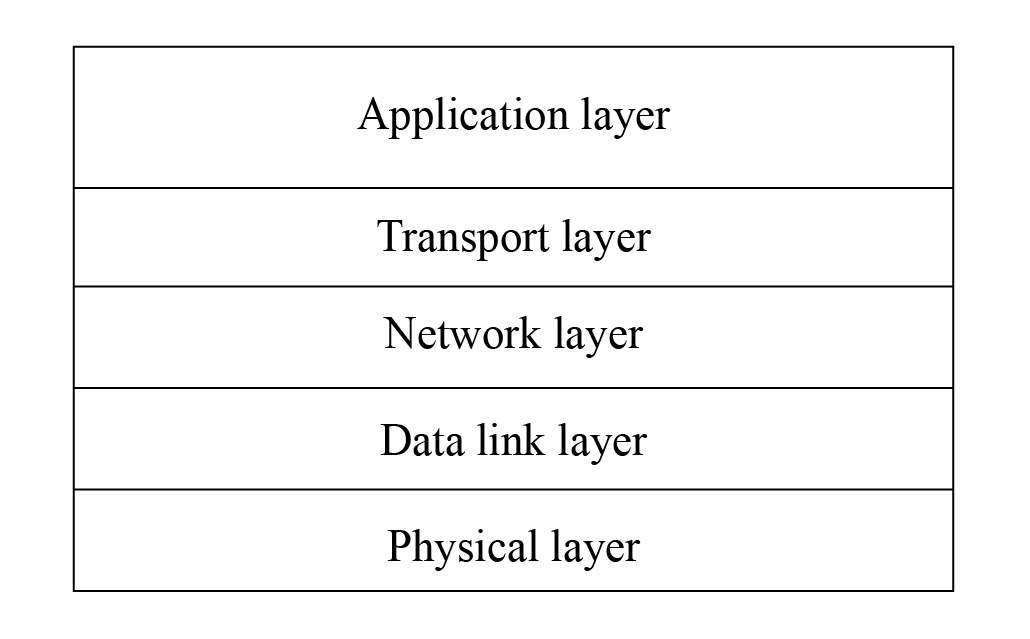
\includegraphics[width=0.5\textwidth]{D8Z/8-2}
    \caption{TCP/IP model}
\end{figure}

\subsubsection{1. Introduction to TCP}
TCP is a connection-oriented, reliable, byte-stream-based communication protocol at the transport layer, defined by RFC 793 of IETF.

\begin{itemize}[leftmargin=1.5em]
    \item \textbf{Connection-oriented}. Before sending data using TCP, a connection must be established between the sender and receiver, which is commonly referred to as a three-way handshake.
    \item \textbf{Reliable}. When sending data using TCP, the receiver’s receipt can be guaranteed. If data is lost, the lost data will be retransmitted. TCP can also ensure that the receiver receives data in order.
    \item \textbf{Byte-stream-based}. When sending data using TCP, the application layer data is first written into the TCP buffer. Then, TCP controls the transmission of data in a byte-stream-based manner, which is independent of the length of the message written by the application layer. Therefore, it is a byte-stream-based protocol.
\end{itemize}

The process of TCP sending upper-layer application data to the receiver is as follows:

\begin{enumerate}[label=(\arabic*)]
    \item The upper-layer application program writes the application data into the TCP buffer.
    \item The TCP buffer packages the data into a TCP message and sends it to the network layer.
    \item The receiver receives the TCP message and puts it into the TCP buffer.
    \item After a certain amount of data is received, the data is sorted and reorganised before being reported to the application layer.
\end{enumerate}

The process of sending and receiving data using TCP is shown in Figure 8.3.

\begin{figure}[!h]
    \centering
    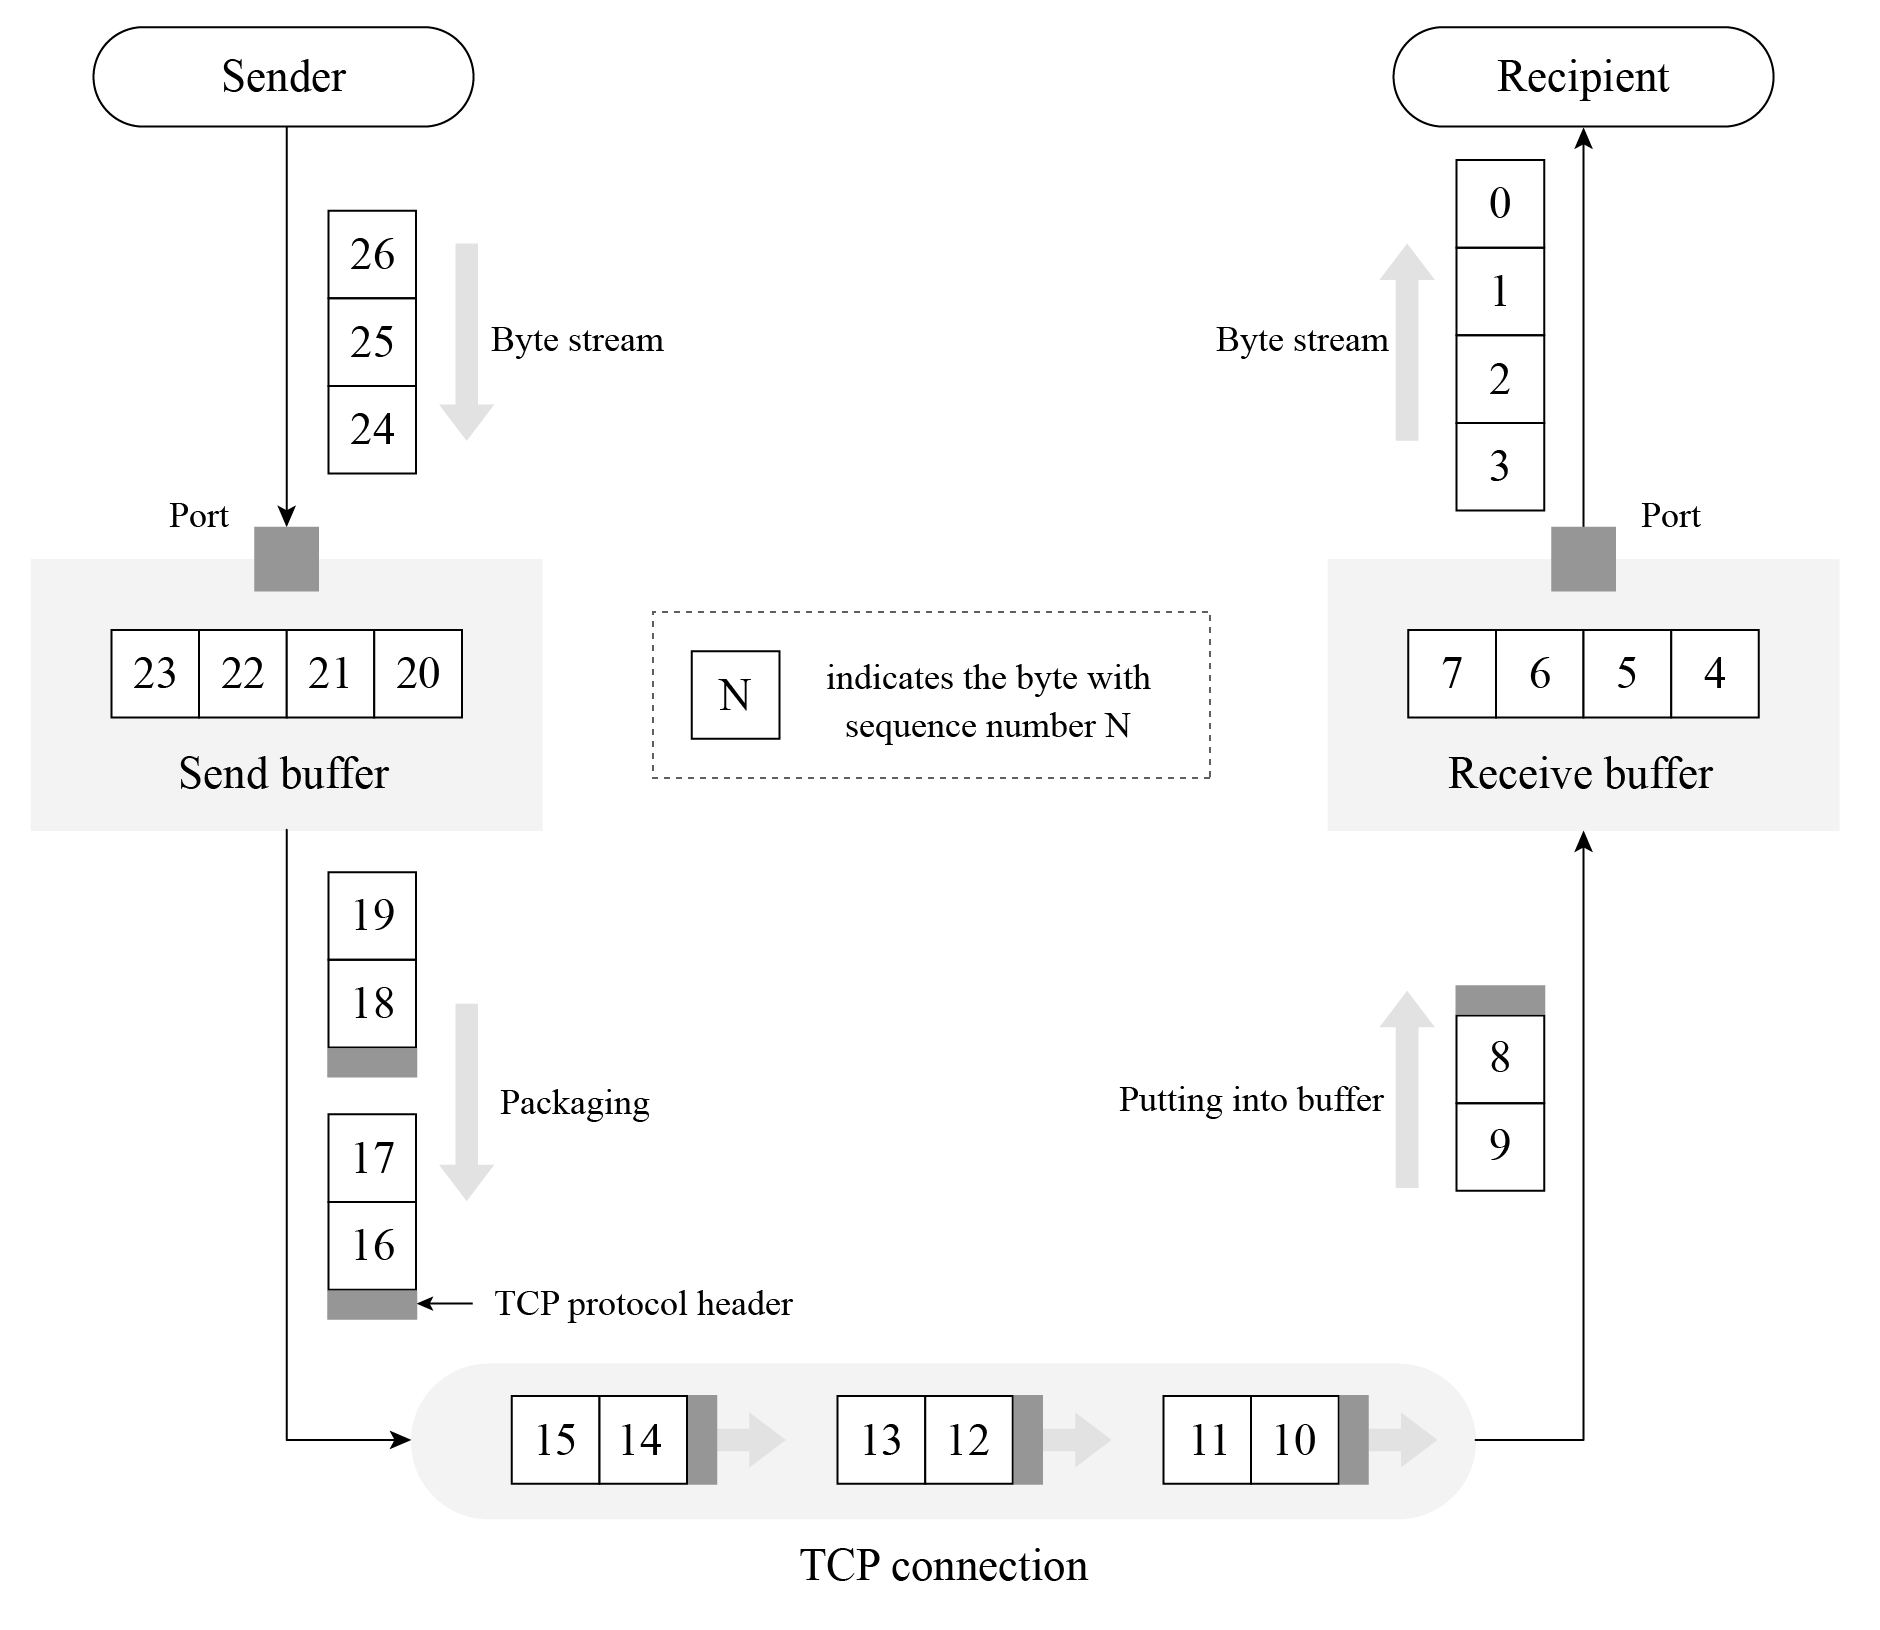
\includegraphics[width=0.8\textwidth]{D8Z/8-3}
    \caption{Data sending and receiving process using TCP}
\end{figure}

\subsubsection{2. Creating a TCP server using socket}
\note[Source code]{For the source code of the function \texttt{esp\_create\_tcp\_server()}, please refer to \href{https://github.com/espressif/book-esp32c3-iot-projects/tree/main/test_case/tcp_socket}{\texttt{book-\newline esp32c3-iot-projects/test\_case/tcp\_socket}}.}

The function \verb|esp_create_tcp_server()| can create a TCP server, including creating a TCP socket, configuring and binding the port, listening, receiving data, and sending data. Compared with TCP clients, UDP servers and clients, the code flow of TCP servers is more complicated, and involves two socket functions, \verb|listen| and \verb|accept|, which are unique to TCP servers. The code is as below:

\begin{codebloc}
\begin{tabular}{d}
\vspace{2pt}
\begin{verbatim}
1.  esp_err_t esp_create_tcp_server(void)
2.  {
3.    int len;
4.    int keepAlive = 1;
5.    int keepIdle = 5;
6.    int keepInterval = 5;
7.    int keepCount = 3;
8.    char rx_buffer[128] = {0};
9.    char addr_str[32] = {0};
10.   esp_err_t err = ESP_FAIL;
11.   struct sockaddr_in server_addr;
12.	
13.   //Create a TCP socket
14.   int listenfd = socket(AF_INET, SOCK_STREAM, 0);
15.   if (listenfd < 0) {
16.     ESP_LOGE(TAG, "create socket error");
17.     return err;
\end{verbatim}
\verb|18.   }|
\end{tabular}
\end{codebloc}

\begin{codebloc}
\begin{tabular}{d}
\vspace{2pt}
\begin{verbatim}
19.     ESP_LOGI(TAG, "create socket success, listenfd : %d", listenfd);
20.	
21.   //Enable SO_REUSEADDR, allowing the server to bind the connected address
22.   int opt = 1;
23.   int ret = setsockopt(listenfd, SOL_SOCKET, SO_REUSEADDR, &opt,
24.                       sizeof(opt));
25.   if (ret < 0) {
26.     ESP_LOGE(TAG, "Failed to set SO_REUSEADDR. Error %d", errno);
27.     goto exit;
28.   }
29.	
\end{verbatim}
\verb|30. |\fontsize{9.5pt}{10pt}\selectfont//Bind the server to an interface with all-zero IP address and port number 3333
\footnotesize
\begin{verbatim}
31.   server_addr.sin_family = AF_INET;
32.   server_addr.sin_addr.s_addr = INADDR_ANY;
33.   server_addr.sin_port = htons(3333);
\end{verbatim}
\verb|34.   |\fontsize{9.5pt}{10pt}\selectfont\verb|ret = bind(listenfd, (struct sockaddr *) &server_addr, sizeof(server_addr));|
\footnotesize
\begin{verbatim}
35.   if (ret < 0) {
36.     ESP_LOGE(TAG, "bind socket failed, socketfd: %d, errno : %d",
37.             listenfd, errno);
38.     goto exit;
39.   }
40.   ESP_LOGI(TAG, "bind socket success");
41.   ret = listen(listenfd, 1);
42.   if (ret < 0) {
43.     ESP_LOGE(TAG, "listen socket failed, socketfd : %d, errno : %d",
44.             listenfd, errno);
45.     goto exit;
46.   }
47.   ESP_LOGI(TAG, "listen socket success");
48.   while (1) {
49.     struct sockaddr_in source_addr;
50.     socklen_t addr_len = sizeof(source_addr);
51.	
\end{verbatim}
\verb|52. |\fontsize{9.5pt}{10pt}\selectfont\verb|//Wait for new TCP connection, and return the communicating socket with the peer|
\footnotesize
\begin{verbatim}
53.     int sock = accept(listenfd, (struct sockaddr *)&source_addr, &addr_len);
54.     if (sock < 0) {
55.        ESP_LOGE(TAG, "Unable to accept connection: errno %d", errno);
56.        break;
57.     }
58.	
59.     //Enable TCP keep-alive function to prevent zombie clients
60.     setsockopt(sock, SOL_SOCKET, SO_KEEPALIVE, &keepAlive, sizeof(int));
61.     setsockopt(sock, IPPROTO_TCP, TCP_KEEPIDLE, &keepIdle, sizeof(int));
62.     setsockopt(sock, IPPROTO_TCP, TCP_KEEPINTVL,&keepInterval, sizeof(int));
63.     setsockopt(sock, IPPROTO_TCP, TCP_KEEPCNT, &keepCount, sizeof(int));
64.     if (source_addr. sin_family == PF_INET) {
\end{verbatim}
\verb|65.        inet_ntoa_r(((struct sockaddr_in *)&source_addr)->sin_addr,|
\end{tabular}
\end{codebloc}

\begin{codebloc}
\begin{tabular}{d}
\vspace{2pt}
\begin{verbatim}
66.                   addr_str, sizeof(addr_str) - 1);
67.     }
68.     ESP_LOGI(TAG, "Socket accepted ip address: %s", addr_str);
69.     do {
70.        len = recv(sock, rx_buffer, sizeof(rx_buffer) - 1, 0);
71.        if (len < 0) {
72.           ESP_LOGE(TAG, "Error occurred during receiving: errno %d", errno);
73.        } else if (len == 0) {
74.           ESP_LOGW(TAG, "Connection closed");
75.        } else {
76.           rx_buffer[len] = 0;
77.           ESP_LOGI(TAG, "Received %d bytes: %s", len, rx_buffer);
78.        }
79.     } while (len > 0);
80.     shutdown(sock, 0);
81.     close(sock);
82.   }
83.	exit:
84.   close(listenfd);
85.   return err;
\end{verbatim}
\verb|86.	}|
\end{tabular}
\end{codebloc}

The above code creates a TCP server and listens to the application data on port 3333. The socket option \verb|SO_REUSEADDR| allows the server to bind to the address of an already established connection, which is useful for the code on the server side. The socket option \verb|SO_KEEPALIVE| enables the TCP keep-alive function, which can detect some abnormally disconnected clients and prevent them from occupying server processes. Socket options \verb|TCP_KEEPIDLE|, \verb|TCP_KEEPINTVL| and \verb|TCP_KEEPCNT| correspond to the idle time since the last data sent by the peer, the interval time for sending TCP keep-alive messages, and the maximum number of retries for sending messages, respectively. For example, if a TCP client sets \verb|TCP_KEEPIDLE| to 5, it means that if there is no data communication between the client and the server within 5 seconds, the client needs to send a TCP keep-alive message to the server; if the client sets \verb|TCP_KEEPINTVL| to 5, it means that if the client sends a TCP keep-alive message to the server and the server does not reply within 5 seconds, the client needs to resend the message to the server; if the client sets \verb|TCP_KEEPCNT| to 3, it means that the client can retry sending the TCP keep-alive message to the server for a maximum of 3 times.

\subsubsection{3. Creating a TCP client using socket}
\note[Source code]{For the source code of the function \texttt{esp\_create\_tcp\_client()}, please refer to \href{https://github.com/espressif/book-esp32c3-iot-projects/tree/main/test_case/tcp_socket}{\texttt{book-\newline esp32c3-iot-projects/test\_case/tcp\_socket}}.}

The function \verb|esp_create_tcp_client()| can create a TCP connection between a TCP client and a server, including creating of a TCP socket, configuring the destination address and port, connecting, and sending data. The code is as below:

\begin{codebloc}
\begin{tabular}{d}
\vspace{2pt}
\begin{verbatim}
1.  #define HOST_IP "192.168.3.80"
2.  #define PORT 3333
3.	
4.  esp_err_t esp_create_tcp_client(void)
5.  {
6.      esp_err_t err = ESP_FAIL;
7.      char *payload = "Open the light";
8.      struct sockaddr_in dest_addr;
9.      dest_addr.sin_addr.s_addr = inet_addr(HOST_IP);
10.     dest_addr.sin_family = AF_INET;
11.     dest_addr.sin_port = htons(PORT);
12.	
13.     //Create a TCP socket
14.     int sock = socket(AF_INET, SOCK_STREAM, 0);
15.     if (sock < 0) {
16.        ESP_LOGE(TAG, "Unable to create socket: errno %d", errno);
17.        return err;
18.     }
19.     ESP_LOGI(TAG, "Socket created, connecting to %s:%d", HOST_IP, PORT);
20.	
21.     //Connect to the TCP server
\end{verbatim}
\verb|22.     |\fontsize{9.5pt}{10pt}\selectfont\verb|int ret = connect(sock, (struct sockaddr *)&dest_addr, sizeof(dest_addr));|
\footnotesize
\begin{verbatim}
23.     if (ret ! = 0) {
24.         ESP_LOGE(TAG, "Socket unable to connect: errno %d", errno);
25.         close(sock);
26.         return err;
27.     }
28.     ESP_LOGI(TAG, "Successfully connected");
29.	
30.     //Send TCP data
31.     ret = send(sock, payload, strlen(payload), 0);
32.     if (ret < 0) {
33.         ESP_LOGE(TAG, "Error occurred during sending: errno %d", errno);
34.         goto exit;
35.     }
36.     err = ESP_OK;
37. exit:
38.     shutdown(sock, 0);
39.     close(sock);
40.     return err;
\end{verbatim}
\verb|41. }|
\end{tabular}
\end{codebloc}

After the client establishes a TCP connection with the server, it sends the TCP data “Open the light” to the server. In addition to using TCP sockets, the client can also use TCP debugging tools to simulate the client for TCP connection.

Based on the above TCP client and server code, and combined with the requirement of controlling the smart light through a smartphone, you can implement code of TCP server on the smart light device and code of TCP client on the smartphone. After establishing a TCP connection between the smartphone and the smart light, the smartphone can send data. For example, in the above code, the TCP client sends the data “Open the light”; and after the smart light receives the data, it can turn on the light by pulling up the GPIO pin level of the smart light.

\subsection{HyperText Transfer Protocol (HTTP)}
HTTP is an application protocol based on the transport layer. It is the data communication foundation of the World Wide Web (WWW or Web), which specifies the format and method of data transmission between clients and servers. Clients can use HTTP to obtain the on/off status of the smart light (GET) or turn the smart light on and off (POST) through HTTP requests, and each operation will have a response from the peer. Therefore, HTTP is completer and more reasonable in applications than simple TCP.

\subsubsection{1. Introduction to HTTP}
HTTP is a standard for requests and responses between clients (users) and servers (websites). The client establishes a TCP connection with the server through a web browser, web crawler or other tools, and then sends requests to read server data, upload data or forms to the server, and read the response status of the server, such as “HTTP/1.1 200 OK”, as well as the returned content (such as requested files, error messages or other information). Resources requested through HTTP are identified by uniform resource identifiers (URIs).

In versions 0.9 and 1.0 of HTTP, the TCP connection is closed after each request and response. In version 1.1 of HTTP, a mechanism for maintaining the connection was introduced, allowing a connection to repeat multiple requests and responses, reducing TCP handshake time and network overhead before each data request.

Common HTTP request methods include:

\begin{itemize}[noitemsep]
    \item \textbf{GET}: Request the specified URI resource.
    \item \textbf{POST}: Submit data to the specified URI resource and request the server to process it (such as submitting a form or uploading a file).
    \item \textbf{DELETE}: Request the server to delete the resource identified by the URI.
\end{itemize}

For local control of smart lights, you can use the GET method to obtain their status, and use the POST method to control them.

\subsubsection{2. Creating an HTTP server using ESP-IDF component}
\note[Source code]{For the source code of the function \texttt{esp\_start\_webserver()}, please refer to \href{https://github.com/espressif/book-esp32c3-iot-projects/tree/main/test_case/https_server}{\texttt{book-esp\newline 32c3-iot-projects/test\_case/https\_server}}.}

The function \verb|esp_start_webserver()| can create an HTTP server. The callback functions corresponding to the GET and POST operations on the server side are defined as \verb|esp_light_get_handler()| and \verb|esp_light_set_handler()| respectively, and must be registered through the function \verb|httpd_register_uri_handler()| after calling the function \verb|httpd_start()| on the server side.

\begin{codebloc}
\begin{tabular}{d}
\vspace{2pt}
\begin{verbatim}
1.  char buf[100] = "{\\"status\\": true}";
2.  //Callback function of the HTTP GET request
3.  esp_err_t esp_light_get_handler(httpd_req_t *req)
4.  {
5.      //Send data in JSON containing the status of smart lights to the client
6.      httpd_resp_send(req, buf, strlen(buf));
7.      return ESP_OK;
8.  }
9.	
10. //Callback function of the HTTP POST request
11. esp_err_t esp_light_set_handler(httpd_req_t *req)
12. {
13.     int ret, remaining = req->content_len;
14.     memset(buf, 0 , sizeof(buf));
15.     while (remaining > 0) {
16.         //Read HTTP request data
17.         if ((ret = httpd_req_recv(req, buf, remaining)) <= 0) {
18.             if (ret == HTTPD_SOCK_ERR_TIMEOUT) {
19.                 continue;
20.             }
21.             return ESP_FAIL;
22.         }
23.         remaining -= ret;
24.     }
25.     ESP_LOGI(TAG, "%.*s", req->content_len, buf);
26.	
27.     //TODO: Read and parse the data; then control the smart light
28.     return ESP_OK;
29. }
30.	
31. //Callback function corresponding to GET
32. static const httpd_uri_t status = {
33.     .uri = "/light",
\end{verbatim}
\verb|34.     .method = HTTP_GET,|
\end{tabular}
\end{codebloc}

\begin{codebloc}
\begin{tabular}{d}
\vspace{2pt}
\begin{verbatim}
35.     .handler = esp_light_get_handler,
36. };
37.	
38. //Callback function corresponding to POST
39. static const httpd_uri_t ctrl = {
40.     .uri = "/light",
41.     .method = HTTP_POST,
42.     .handler = esp_light_set_handler,
43. };
44.	
45. esp_err_t esp_start_webserver()
46. {
47.     httpd_handle_t server = NULL;
48.     httpd_config_t config = HTTPD_DEFAULT_CONFIG();
49.     config.lru_purge_enable = true;
50.	
51.     //Start the HTTP server
52.     ESP_LOGI(TAG, "Starting server on port: '%d'", config. server_port);
53.     if (httpd_start(&server, &config) == ESP_OK) {
54.         //Set the callback function corresponding to the HTTP URI
55.         ESP_LOGI(TAG, "Registering URI handlers");
56.         httpd_register_uri_handler(server, &status);
57.         httpd_register_uri_handler(server, &ctrl);
58.         return ESP_OK;
59.     }
60.     ESP_LOGI(TAG, "Error starting server!" );
61.     return ESP_FAIL;
\end{verbatim}
\verb|62. }|
\end{tabular}
\end{codebloc}

The above code implements an HTTP server for querying and setting the status of the smart light. When accessing \verb|http://[ip]/light| through a browser, the browser will return \verb|{"status": true}| (as shown in Figure 8.4) or \verb|{"status": false}| to indicate the status of the smart light.

\begin{figure}[!h]
    \centering
    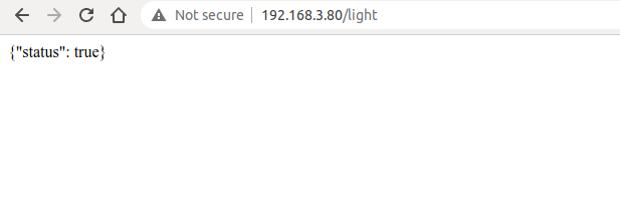
\includegraphics[width=0.75\textwidth,frame]{D8Z/8-4}
    \caption{Using HTTP to query the status of the smart light}
\end{figure}

Press F12 on the current page to enter the Console. Enter the following command and press “Enter” to send a POST request.

\begin{codebloc}
\begin{tabular}{d}
\$ \textbf{var xhr = new XMLHttpRequest();}

\$ \textbf{xhr.open("POST", "192.168.3.80/light", true);}

\$ \textbf{xhr.send("\{\textbackslash"status\textbackslash": false\}");}
\end{tabular}
\end{codebloc}

Figure 8.5 shows how to use HTTP to set the status of the smart light.

\begin{figure}[!h]
    \centering
    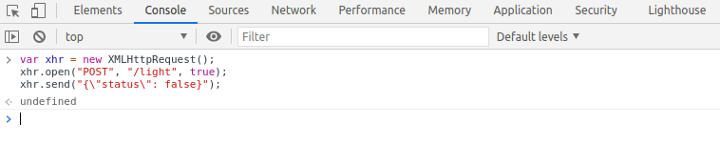
\includegraphics[width=0.65\textwidth,frame]{D8Z/8-5}
    \caption{Using HTTP to set the status of the smart light}
\end{figure}

At this point, the server will receive the HTTP POST request \verb|{"status": false}|. The log of using HTTP to set the status of the smart light is as follows:

\begin{codebloc}
\begin{tabular}{d}
\vspace{2pt}
\begin{verbatim}
I (773) wifi:mode:sta (30:ae:a4:80:48:98)
I (773) wifi:enable tsf 
I (773) wifi station: wifi init sta finished. 
I (793) wifi:new: <6,0>, old: <1,0>, ap: <255,255>, sta: <6,0>, prof:1 
I (793) wifi:state: init -> auth (be) 
I (813) wifi:state: auth -> assoc (0) 
I (823) wifi:state: assoc -> run (10) 
I (873) wifi:connected with myssid, aid = 1, channel 6, BW20, bssid = 
34:29:12:43:c5:40
I (873) wifi:security: WPA2-PSK, phy: bgn, rssi: -21 
I (883) wifi:pm start, type: 1 
I (943) wifi:AP's beacon interval = 102400 us, DTIM period = 1 
I (1543) esp netif handlers: sta ip: 192.168.3.80, mask: 255.255.255.0, gw: 192.
168.3.1
I (1543) wifi station: got ip:192.168.3.80
I (1543) wifi station: connected to ap SSID: myssid password: 12345678
I (1553) wifi station: Starting server on port: '80'
I (1563) wifi station: Registering URI handlers 
W (11393) wifi:<ba-add>idx:0 (ifx:0,34:29:12:43:c5:40), tid:7, ssn:4, winSize:64
\end{verbatim}
\verb|I (11413) wifi station: {"status": false}|
\end{tabular}
\end{codebloc}

Refreshing the current page at this time can continue to query the status of the smart light, and the previously set status will be displayed, as shown in Figure 8.6.

\begin{figure}[!h]
    \centering
    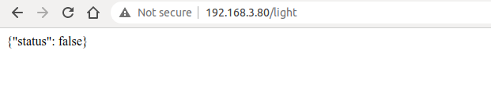
\includegraphics[width=0.65\textwidth,frame]{D8Z/8-6}
    \caption{Displaying the modified status of the smart light}
\end{figure}

\subsection{User Datagram Protocol (UDP)}
Subsections 8.3.1 and 8.3.2 respectively introduce TCP and HTTP, both of which are characterised by reliable transmission. This subsection will introduce another protocol at the transport layer, UDP. Unlike TCP, UDP is an unreliable transmission protocol. Common application protocols based on UDP include DNS, TFTP, and SNMP.

\subsubsection{1. Introduction to UDP}
UDP is a simple datagram-oriented communication protocol, which is located at the transport layer like TCP. UDP was designed by David P. Reed in 1980 and defined in RFC 768 (excerpted from Wikipedia). UDP is an unreliable transmission protocol. After data is sent through UDP, the underlying layer does not retain the data to prevent loss during transmission. UDP itself does not support error correction, queue management, or congestion control, but supports checksums.

UDP is a connectionless protocol. It does not need to establish a connection before sending data, unlike TCP. Data can be sent directly to the peer without establishing a connection. Because no connection needs to be established during data transmission, there is no need to maintain connection status, including sending and receiving status.

UDP is only responsible for transmission, so applications that use this protocol need to do more control over how data is sent and processed, such as how to ensure that peer’s applications receive the data correctly and in order.

Compared with TCP, UDP cannot guarantee the safe and reliable transmission of data. You may wonder why the UDP protocol is still used. The connectionless nature of UDP results in less network and time overhead than TCP. The unreliable transmission of UDP (mainly the inability to guarantee retransmission after packet loss) is more suitable for applications such as streaming media, real-time multiplayer games, and IP voice, where losing a few packets will not affect the application. On the other hand, if TCP is used for retransmission, it will greatly increase network latency.

\subsubsection{2. Creating a UDP server using socket}
\note[Source code]{For the source code of the function \texttt{esp\_create\_udp\_server()}, please refer to \href{https://github.com/espressif/book-esp32c3-iot-projects/tree/main/test_case/udp_socket}{\texttt{book-\newline esp32c3-iot-projects/test\_case/udp\_socket}}.}

Creating a UDP server using socket is similar to creating a multicast group receiver as introduced in subsection 8.2.2. Both involve creating a UDP socket, configuring the bound port, and receiving and sending data. The function \verb|esp_create_udp_server()| sets the \verb|SO_REUSEADDR| option, allowing the server to bind the address of the already established connection. The code is as below:

\begin{codebloc}
\begin{tabular}{d}
\vspace{2pt}
\begin{verbatim}
1.  esp_err_t esp_create_udp_server(void)
2.  {
3.      char rx_buffer[128];
4.      char addr_str[32];
5.      esp_err_t err = ESP_FAIL;
6.      struct sockaddr_in server_addr;
7.      //Create a UDP socket
8.      int sock = socket(AF_INET, SOCK_DGRAM, 0);
9.      if (sock < 0) {
10.         ESP_LOGE(TAG, "create socket error");
11.         return err;
12.     }
13.     ESP_LOGI(TAG, "create socket success, sock : %d", sock);
14.     //Enable SO_REUSEADDR, allowing the server to bind connected address
15.     int opt = 1;
16.     int ret = setsockopt(sock, SOL_SOCKET, SO_REUSEADDR, &opt, sizeof(opt));
17.     if (ret < 0) {
18.         ESP_LOGE(TAG, "Failed to set SO_REUSEADDR. Error %d", errno);
19.         goto exit;
20.     }
\end{verbatim}
\verb|21. |\fontsize{9.5pt}{10pt}\selectfont//Bind the server to an interface with all-zero IP address and port number 3333
\footnotesize
\begin{verbatim}
22.     server_addr.sin_family = AF_INET;
23.     server_addr.sin_addr.s_addr = INADDR_ANY;
24.     server_addr.sin_port = htons(PORT);
25.     ret = bind(sock, (struct sockaddr *) &server_addr, sizeof(server_addr));
26.     if (ret < 0) {
\end{verbatim}
\verb|27.         |\fontsize{9pt}{10pt}\selectfont\verb|ESP_LOGE(TAG, "bind socket failed, socketfd: %d, errno : %d", sock, errno);|
\footnotesize
\begin{verbatim}
28.         goto exit;
29.     }
30.     ESP_LOGI(TAG, "bind socket success");
31.     while (1) {
32.         struct sockaddr_in source_addr;
33.         socklen_t addr_len = sizeof(source_addr);
34.         memset(rx_buffer, 0, sizeof(rx_buffer));
35.         int len = recvfrom(sock, rx_buffer, sizeof(rx_buffer) - 1, 0,
36.                             (struct sockaddr *)&source_addr, &addr_len);
37.         // Reception error
38.         if (len < 0) {
39.             ESP_LOGE(TAG, "recvfrom failed: errno %d", errno);
40.             break;
41.         } else { //Data is received
42.             if (source_addr. sin_family == PF_INET) {
43.                 inet_ntoa_r(((struct sockaddr_in *)&source_addr)->sin_addr,
\end{verbatim}
\verb|44.                           addr_str, sizeof(addr_str) - 1);|
\end{tabular}
\end{codebloc}

\begin{codebloc}
\begin{tabular}{d}
\vspace{2pt}
\begin{verbatim}
45.             }
46.             //String ends with NULL
47.             rx_buffer[len] = 0;
48.             ESP_LOGI(TAG, "Received %d bytes from %s:" , len, addr_str);
49.             ESP_LOGI(TAG, "%s", rx_buffer);
50.         }
51.     }
52. exit:
53.     close(sock);
54.     return err;
\end{verbatim}
\verb|55. }|
\end{tabular}
\end{codebloc}

\subsubsection{3. Creating a UDP client using socket}
\note[Source code]{For the source code of the function \texttt{esp\_create\_udp\_client()}, please refer to \href{https://github.com/espressif/book-esp32c3-iot-projects/tree/main/test_case/udp_socket}{\texttt{book-\newline esp32c3-iot-projects/test\_case/udp\_socket}}.}

With the function \verb|esp_create_udp_client()|, the UDP client can send data, including creating UDP sockets, configuring destination addresses and ports, calling socket interface \verb|sendto()| to send data. The code is as below:

\begin{codebloc}
\begin{tabular}{d}
\vspace{2pt}
\begin{verbatim}
1.  esp_err_t esp_create_udp_client(void)
2.  {
3.      esp_err_t err = ESP_FAIL;
4.      char *payload = "Open the light";
5.      struct sockaddr_in dest_addr;
6.      dest_addr.sin_addr.s_addr = inet_addr(HOST_IP);
7.      dest_addr.sin_family = AF_INET;
8.      dest_addr.sin_port = htons(PORT);
9.	
10.     //Create a UDP socket
11.     int sock = socket(AF_INET, SOCK_DGRAM, 0);
12.     if (sock < 0) {
13.         ESP_LOGE(TAG, "Unable to create socket: errno %d", errno);
14.         return err;
15.     }
16. 	 
17.     //Send data
18.     int ret = sendto(sock, payload, strlen(payload), 0,
19.                     (struct sockaddr *)&dest_addr, sizeof(dest_addr));
20.     if (ret < 0) {
21.         ESP_LOGE(TAG, "Error occurred during sending: errno %d", errno);
22.         goto exit;
23.     }
\end{verbatim}
\verb|24.     ESP_LOGI(TAG, "Message send successfully");|
\end{tabular}
\end{codebloc}

\begin{codebloc}
\begin{tabular}{d}
\vspace{2pt}
\begin{verbatim}
25.     err = ESP_OK;
26. exit:
27.     close(sock);
28.     return err;
\end{verbatim}
\verb|29. }|
\end{tabular}
\end{codebloc}

UDP clients do not need to establish a connection with the server, and can directly send data to the server. Since UDP creates unreliable connections, the data sent, such as “Open the light,” may be lost, causing the peer to fail to receive it. Therefore, when writing code for the client and server, some logic should be added to the application layer code to ensure that data is not lost. For example, when the client sends “Open the light” to the server, the server returns “Open the light OK” after receiving it successfully. If the client receives the data within 1 second, it means that the data has been sent to the server correctly. If the client does not receive it within 1 second, it needs to send the data “Open the light” again.

\subsection{Constrained Application Protocol (CoAP)}
With the rapid development of IoT technology, a series of protocols have been created for IoT devices. Most IoT devices have limited resources, such as RAM, flash, CPU, network bandwidth, etc. More memory and network bandwidth are often required if they want to use TCP and HTTP protocols for data transmission. If UDP can be used for data transmission, is there an application protocol similar to HTTP? The answer is yes, CoAP is designed according to the REST architecture of HTTP.

\subsubsection{1. Introduction to CoAP}
CoAP is a protocol similar to web applications in IoT devices. It is defined in RFC 7252 and can be used for resource-constrained IoT devices, allowing those resource-constrained devices called nodes to communicate with a wider range of the Internet using similar protocols. CoAP is designed for devices on the same constrained network (such as low-power, lossy networks), between devices and general nodes on the Internet, and between devices on different constrained networks connected by the Internet.

CoAP is based on the request and response model, similar to HTTP, which can make up for the shortcomings of unreliable transmission of UDP and ensure that data is not lost or disordered. The server’s resources are identified by URLs (such as \verb|coap://[IP]/id/light_|\\ \verb|status|) to access the status of a smart light. The client accesses the server’s resources through the URL of a resource and operate the server’s resources through four request methods (GET, PUT, POST, and DELETE).

CoAP also has the following features:

\begin{itemize}[leftmargin=1.5em,noitemsep]
    \item Both the client and server can independently send requests to each other.
    \item Supports reliable data transmission.
    \item Supports multicast and broadcast, enabling one-to-many data transmission.
    \item Supports communication with low power consumption and non-persistent connections.
    \item Compared with HTTP, its header is lighter.
\end{itemize}

\subsubsection{2. Creating a CoAP server using ESP-IDF component}
The following code shows how to create a CoAP server using ESP-IDF component, which provides GET and PUT operations for resource retrieval and modification in CoAP. CoAP protocol operations are generally fixed, and you only need to focus on your own resource URI paths and the operations you need to provide. The function \verb|coap_resource_init()| can be used to set the URI for resource access, and the function \verb|coap_register_handler()| can be used to register GET and PUT callback functions corresponding to the resource URI.

\note[Source code]{For the source code of the functions \texttt{coap\_resource\_init()} and \texttt{coap\_register\_\newline handler()}, please refer to \href{https://github.com/espressif/book-esp32c3-iot-projects/tree/main/test_case/coap}{\texttt{book-esp32c3-iot-projects/test\_case/coap}}.}

\begin{codebloc}
\begin{tabular}{d}
\vspace{2pt}
\begin{verbatim}
1.  static char buf[100] = "{\"status\": true}";
2.	
3.  //Callback function of GET method in CoAP
4.  static void esp_coap_get(coap_context_t *ctx, coap_resource_t *resource,
5.                          coap_session_t *session, coap_pdu_t *request,
6.                          coap_binary_t *token, coap_string_t *query,
7.                          coap_pdu_t *response)
8.  {
9.      coap_add_data_blocked_response(resource, session, request, response,
10.                                   token, COAP_MEDIATYPE_TEXT_PLAIN, 0,
11.                                   strlen(buf), (const u_char *)buf);
12. }
13.	
14. //Callback function of PUT method in CoAP
15. static void esp_coap_put(coap_context_t *ctx,
16.                         coap_resource_t *resource,
17.                         coap_session_t *session,
18.                         coap_pdu_t *request,
19.                         coap_binary_t *token,
20.                         coap_string_t *query,
21.                         coap_pdu_t *response)
22. {
23.     size_t size;
24.     const unsigned char *data;
25.     coap_resource_notify_observers(resource, NULL);
26.	
27.     //Read the received CoAP protocol data
\end{verbatim}
\verb|28.     (void)coap_get_data(request, &size, &data);|
\end{tabular}
\end{codebloc}

\begin{codebloc}
\begin{tabular}{d}
\vspace{2pt}
\begin{verbatim}
29.     if (size) {
30.         if (strncmp((char *)data, buf, size)) {
31.             memcpy(buf, data, size);
32.             buf[size] = 0;
33.             response->code = COAP_RESPONSE_CODE(204);
34.         } else {
35.             response->code = COAP_RESPONSE_CODE(500);
36.         }
37.     } else { //A size of 0 indicates a receiving error
38.         response->code = COAP_RESPONSE_CODE(500);
39.     }
40. }
41.	
42. static void esp_create_coap_server(void)
43. {
44.     coap_context_t *ctx = NULL;
45.     coap_address_t serv_addr;
46.     coap_resource_t *resource = NULL;
47.     while (1) {
48.         coap_endpoint_t *ep = NULL;
49.         unsigned wait_ms;
50.	
51.         //Create a CoAP server socket
52.         coap_address_init(&serv_addr);
53.         serv_addr.addr.sin6.sin6_family = AF_INET6;
54.         serv_addr.addr.sin6.sin6_port = htons(COAP_DEFAULT_PORT);
55.	
56.         //Create CoAP ctx
57.         ctx = coap_new_context(NULL);
58.         if (!ctx) {
59.             ESP_LOGE(TAG, "coap_new_context() failed");
60.             continue;
61.         }
62.	
63.         //Set the CoAP protocol node
64.         ep = coap_new_endpoint(ctx, &serv_addr, COAP_PROTO_UDP);
65.         if (!ep) {
66.             ESP_LOGE(TAG, "udp: coap_new_endpoint() failed");
67.             goto clean_up;
68.         }
69.	
70.         //Set CoAP protocol resource URI
71.         resource = coap_resource_init(coap_make_str_const("light"), 0);
72.         if (!resource) {
73.             ESP_LOGE(TAG, "coap_resource_init() failed");
74.             goto clean_up;
\end{verbatim}
\verb|75.         }|
\end{tabular}
\end{codebloc}

\begin{codebloc}
\begin{tabular}{d}
76.	

77. \fontsize{8.5pt}{10pt}\selectfont//Register callback functions of GET and PUT methods corresponding to CoAP resource URI
\footnotesize
\begin{verbatim}
78.         coap_register_handler(resource, COAP_REQUEST_GET, esp_coap_get);
79.         coap_register_handler(resource, COAP_REQUEST_PUT, esp_coap_put);
80.	
81.         //Set CoAP GET resource observable
82.         coap_resource_set_get_observable(resource, 1);
83.	
84.         //Add resource to CoAP ctx
85.         coap_add_resource(ctx, resource);
86.         wait_ms = COAP_RESOURCE_CHECK_TIME * 1000;
87.         while (1) {
88.             //Wait to receive CoAP data
89.             int result = coap_run_once(ctx, wait_ms);
90.             if (result < 0) {
91.                 break;
92.             } else if (result && (unsigned)result < wait_ms) {
93.                 //Decrease waiting time
94.                 wait_ms -= result;
95.             } else {
96.                 //Reset waiting time
97.                 wait_ms = COAP_RESOURCE_CHECK_TIME * 1000;
98.             }
99.         }
100.    }
101.clean_up:
102.    coap_free_context(ctx);
103.    coap_cleanup();
\end{verbatim}
\verb|104.}|
\end{tabular}
\end{codebloc}

The above code creates a CoAP server, and provides the GET method to query the status of the smart light and the PUT method to set the status of the smart light. You can use the Chrome browser to install CoAP to debug the client Copper plugin and simulate the CoAP client.

Open the Chrome plugin Copper, enter the \verb|URL coap://[ip]/light|, and press “Enter” to connect to the server. Figure 8.7 shows the connection of the CoAP plugin.

\begin{figure}[!h]
    \centering
    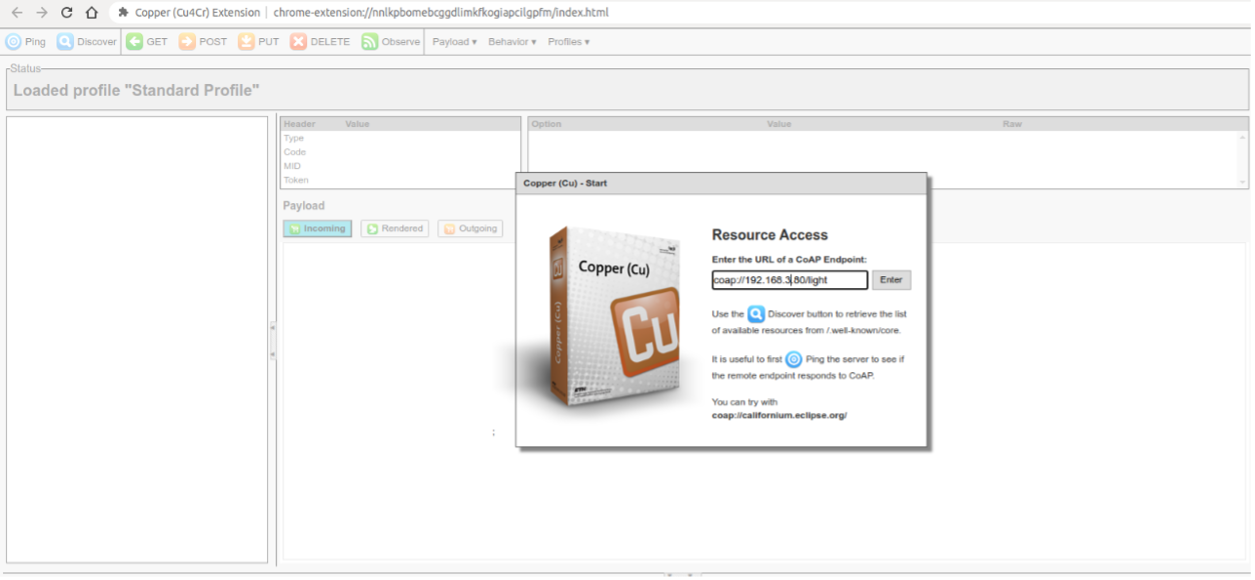
\includegraphics[width=0.75\textwidth]{D8Z/8-7}
    \caption{Connection of CoAP plugin}
\end{figure}

After the connection is successful, click the “GET” button in the upper left corner to get the status and display \verb|{"status": true}|, the query status of CoAP plugin is shown in Figure 8.8.

\begin{figure}[!h]
    \centering
    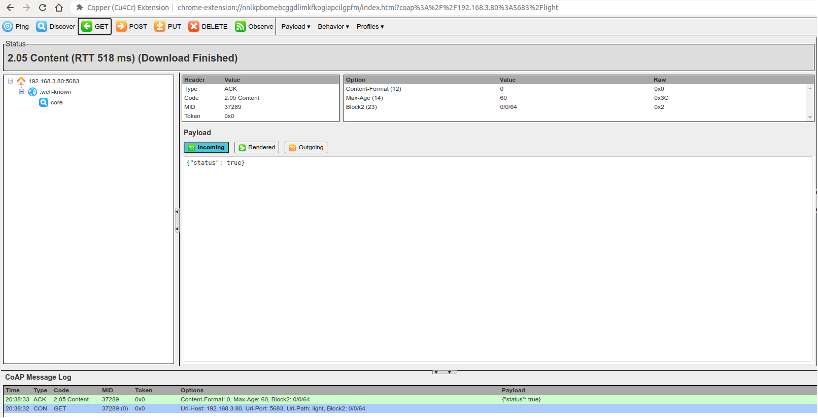
\includegraphics[width=0.75\textwidth]{D8Z/8-8}
    \caption{Query status of CoAP plugin}
\end{figure}

Click the “PUT” button in the upper left corner, and modify the data in “Payload” → “Outgoing” to \verb|{"status": false}| to set the status of the smart light to \verb|false|. Figure 8.9 shows the configuration status of the CoAP plugin.

\begin{figure}[!h]
    \centering
    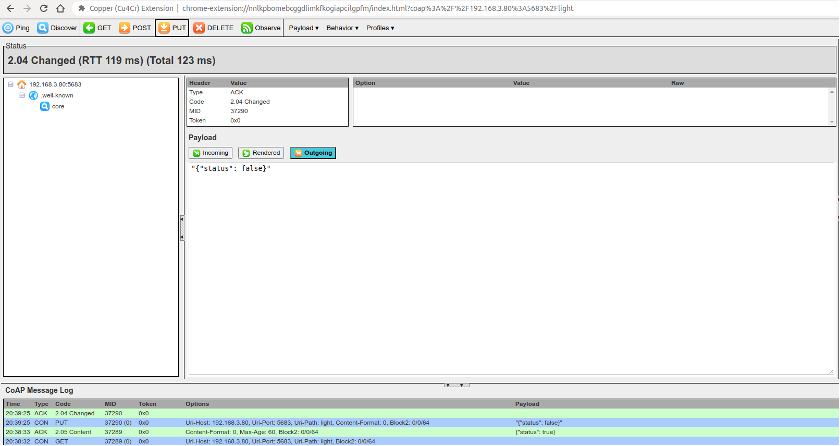
\includegraphics[width=0.75\textwidth]{D8Z/8-9}
    \caption{Setting status of CoAP plugin}
\end{figure}

At this time, click the “GET” button in the upper left corner again to get the status, which displays \verb|{"status": false}|. Figure 8.10 shows the query setting status of the CoAP plugin.

\begin{figure}[!h]
    \centering
    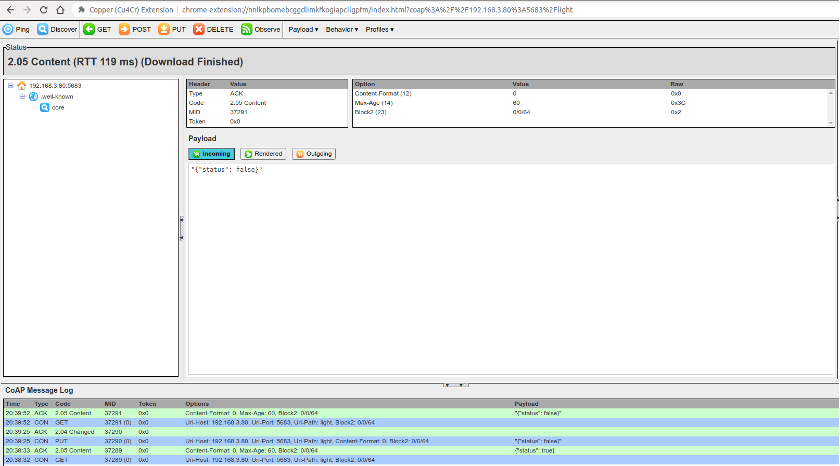
\includegraphics[width=0.75\textwidth]{D8Z/8-10}
    \caption{Query setting status of CoAP plugin}
\end{figure}

\subsection{Bluetooth Protocol}
\subsubsection{1. Introduction to Bluetooth protocol}
Chapter 7 introduces the protocol and architecture of Bluetooth. The Bluetooth protocol defines message formats and process for completing specific functions, such as link control, security services, service information exchange and data transmission. This section only introduces the attribute protocol (ATT) of the Bluetooth protocol specification. Bluetooth data exists in the form of attributes, and each attribute consists of four elements.

\begin{term}{Attribute handle}
    Just as memory addresses are used to find contents in memory, attribute handles can also help find the corresponding attribute. For example, the first attribute handle is 0x0001, the second attribute handle is 0x0002, and so on, up to a maximum of 0xFFFF.
\end{term}

\begin{term}{Attribute UUID}
    Each data represents specific property. For example, a smart light has two basic attributes, one for setting the on/off status, and the other for reading the on/off status.
\end{term}

\begin{term}{Attribute value}
    Attribute value is the information that each attribute carries, while the other three elements are to enable the peer to obtain the attribute value much easier. For example, for a smart light, the attribute value for setting the on/off status can be set to “1” to turn on the light, or to “0” to turn off the light; the attribute value for reading the on/off status can be “1” for the “on” status or “0” for the “off” status.
\end{term}

\begin{term}{Attribute permissions}
    Each attribute has corresponding access restrictions for its own attribute values, such as some attributes are readable, some are writable, and some are readable and writable. The party that owns the data can control the attribute permissions of local data through attribute permissions. For example, the switch attribute permission of the smart light can be set as writable but not readable, and the attribute permission for reading the switch status of the smart light can be set as read-only and not writable.
\end{term}

Table 8.2 lists the Bluetooth attributes for the basic functions of a smart light.

\begin{table}[h!]
    \renewcommand{\arraystretch}{1.4}
    \caption{Bluetooth attributes for basic functions of smart light}
    \begin{tabular}{|>{\Centering}m{6em}|>{\Centering}m{10em}|>{\Centering}m{6em}|>{\Centering}m{16em}|}
        \hline
        \rowcolor{LightBlue} \textbf{Attribute handle}&\textbf{Attribute UUID}&\textbf{Attribute value}&\textbf{Attribute permissions}\\
        \hline
        0x0001&Set the on/off status&1/0&Writable but not readable\\
        \hline
        0x0002&Read the on/off status&1/0&Readable but not writable\\
        \hline
    \end{tabular}
\end{table}

The device that stores the data (i.e., attributes) is usually called the \textbf{server}, and the device that receives data from other devices is called the \textbf{client}. For a smart light and a smartphone, the smart light is server, and the smartphone is the client. The following are common operations between a server and a client:

\begin{enumerate}[label=(\arabic*)]
    \item The client sends data to the server.
    
    Data is transmitted by writing data to the server. There are two types of write operations: one is \textbf{write request}, and the other is \textbf{write command}. The main difference between the two is that the former requires a response (\textbf{write response}) from the peer, while the latter does not. For a smart light, the command to turn on/off the light sent by the smartphone is a write operation, and this is a write request which requires the smart light to respond. Such response is not a simple ACK response. The result of the action of turning on/off the light needs to be returned to the smartphone to inform it of the current status of the smart light.
    \item The server sends data to the client.
    
    The updated data is sent from the server to the client mainly in the form of server \textbf{indication} or \textbf{notification}. Similar to write operations, the main difference between indication and notification is that the former requires the other device to respond (\textbf{confirm}) after receiving the data indication. For a smart light, if it is turned on/off through a physical switch button, its status needs to be reported to the smartphone through indications or notifications, and the smartphone will display the latest status.
    \item The client reads data from the server actively.
    
    Generally, the client obtains values of corresponding attributes from the server through \textbf{read operation}. In the case mentioned above where a smart light is turned on/off through a physical switch button, except for waiting to be notified by the server, the smartphone can also obtain the real-time status through read operations.
\end{enumerate}

Then let’s consider which way is better to get the status of the smart light. Active reading takes time whenever the smartphone initiates a read operation, while indication or notification saves the time for repetitive data transmission. It seems that the latter option is faster but if the smart light is not connected to the phone when sending the notification, its status will not be updated. This can be fixed by updating the status as soon as the phone becomes connected to the smart light; otherwise, it is recommended to use the read operation.

\subsubsection{2. Creating a Bluetooth server using ESP-IDF component}
\note[Source code]{For the source code of Bluetooth, please refer to \href{https://github.com/espressif/esp-idf/tree/master/examples/provisioning}{\texttt{esp-idf/examples/provisioning/\newline legacy/ble\_prov}}. For the example code of customised configuration, please refer to \href{https://github.com/espressif/esp-idf/tree/master/examples/provisioning}{\texttt{esp-idf/examples/provisioning/legacy/custom\_config}}.}

The following example uses the \verb|protocomm| component to implement the smart light server, and the customised configuration uses the custom-proto protocol. As mentioned earlier, to implement the on/off control and status query of the smart light, two attributes need to be defined. The code is as below:

\begin{codebloc}
\begin{tabular}{d}
\vspace{2pt}
\begin{verbatim}
1.  static esp_err_t wifi_prov_config_set_light_handler(uint32_t session_id,
2.                                                      const uint8_t *inbuf,
3.                                                      ssize_t inlen,
4.                                                      uint8_t **outbuf,
5.                                                      ssize_t *outlen,
6.                                                      void *priv_data)
7.  {
8.      CustomConfigRequest *req;
9.      CustomConfigResponse resp;
10.     req = custom_config_request_unpack(NULL, inlen, inbuf);
11.     if (!req) {
12.         ESP_LOGE(TAG, "Unable to unpack config data");
13.         return ESP_ERR_INVALID_ARG;
14.     }
15.     custom_config_response_init(&resp);
16.     resp.status = CUSTOM_CONFIG_STATUS_ConfigFail;
17.     if (req->open_light) {//Turn on the smart light
18.         //Pull up GPIO level according to the status
\end{verbatim}
\verb|19.         ESP_LOGI(TAG, "Open the light");|
\end{tabular}
\end{codebloc}

\begin{codebloc}
\begin{tabular}{d}
\vspace{2pt}
\begin{verbatim}
20.     } else {
21.         //Pull down GPIO level according to the status
22.         ESP_LOGI(TAG, "Close the light");
23.     }
24.	
\end{verbatim}
25. \fontsize{8.5pt}{10pt}\selectfont//Set response status and smart light status according to the light’s execution result
\footnotesize
\begin{verbatim}
26.     resp.status = CUSTOM_CONFIG_STATUS_ConfigSuccess;
27.     custom_config_request_free_unpacked(req, NULL);
28.     resp.light_status = 1; //Respond according to the light status
29.     *outlen = custom_config_response_get_packed_size(&resp);
30.     if (*outlen <= 0) {
31.         ESP_LOGE(TAG, "Invalid encoding for response");
32.         return ESP_FAIL;
33.     }
34.     *outbuf = (uint8_t *) malloc(*outlen);
35.     if (*outbuf == NULL) {
36.         ESP_LOGE(TAG, "System out of memory");
37.         return ESP_ERR_NO_MEM;
38.     }
39.	
40.     custom_config_response_pack(&resp, *outbuf);
41.     return ESP_OK;
42. }
43.	
44. static int wifi_prov_config_get_light_handler(uint32_t session_id,
45.                                               const uint8_t *inbuf,
46.                                               ssize_t inlen,
47.                                               uint8_t **outbuf,
48.                                               ssize_t *outlen,
49.                                               void *priv_data)
50. {
51.     CustomConfigResponse resp;
52.     custom_config_response_init(&resp);
53.     resp.status = CUSTOM_CONFIG_STATUS_ConfigSuccess;
54.     resp.light_status = 1; //Respond according to the light status
55.     *outlen = custom_config_response_get_packed_size(&resp);
56.     if (*outlen <= 0) {
57.         ESP_LOGE(TAG, "Invalid encoding for response");
58.         return ESP_FAIL;
59.     }
60.     *outbuf = (uint8_t *) malloc(*outlen);
61.     if (*outbuf == NULL) {
62.         ESP_LOGE(TAG, "System out of memory");
63.         return ESP_ERR_NO_MEM;
64.     }
65.     custom_config_response_pack(&resp, *outbuf);
\end{verbatim}
\verb|66.     return ESP_OK;|
\end{tabular}
\end{codebloc}

\begin{codebloc}
\begin{tabular}{d}
\vspace{2pt}
\begin{verbatim}
67. }
68.	
69. static esp_err_t app_prov_start_service(void)
70. {
71.     //Create protocomm
72.     g_prov->pc = protocomm_new();
73.     if (g_prov->pc == NULL) {
74.         ESP_LOGE(TAG, "Failed to create new protocomm instance");
75.         return ESP_FAIL;
76.     }
77.	
78.     //Attribute value
79.     protocomm_ble_name_uuid_t nu_lookup_table[] = {
80.         {"prov-session", 0x0001},
81.         {"prov-config", 0x0002},
82.         {"proto-ver", 0x0003},
83.         {"set-light", 0x0004}, //Set the state of the smart light
84.         {"get-light", 0x0005}, //Get the status of the smart light
85.     };
86.	
87.     //Bluetooth configuration
88.     protocomm_ble_config_t config = {
89.         .service_uuid = {
90.             /* LSB <---------------------------------------
91.             * ---------------------------------------> MSB */
92.             0xb4, 0xdf, 0x5a, 0x1c, 0x3f, 0x6b, 0xf4, 0xbf,
93.             0xea, 0x4a, 0x82, 0x03, 0x04, 0x90, 0x1a, 0x02,
94.         },
95.         .nu_lookup_count=sizeof(nu_lookup_table)/sizeof(nu_lookup_table[0]),
96.         .nu_lookup = nu_lookup_table
97.     };
98.	
99.     uint8_t eth_mac[6];
100.    esp_wifi_get_mac(WIFI_IF_STA, eth_mac);
101.    snprintf(config.device_name,
102.            sizeof(config.device_name),
103.            "%s%02X%02X%02X",
104.            ssid_prefix,
105.            eth_mac[3],
106.            eth_mac[4],
107.            eth_mac[5]);
108.
109.    //Release BT memory as only Bluetooth LE protocol stack is used.
110.    esp_err_t err = esp_bt_controller_mem_release(ESP_BT_MODE_CLASSIC_BT);
111.    if (err) {
112.        ESP_LOGE(TAG, "bt_controller_mem_release failed %d", err);
\end{verbatim}
\verb|113.        if (err ! = ESP_ERR_INVALID_STATE) {|
\end{tabular}
\end{codebloc}

\begin{codebloc}
\begin{tabular}{d}
\vspace{2pt}
\begin{verbatim}
114.            return err;
115.        }
116.    }
117.    //Start protocomm Bluetooth LE protocol stack
118.    if (protocomm_ble_start(g_prov->pc, &config) ! = ESP_OK) {
119.        ESP_LOGE(TAG, "Failed to start BLE provisioning");
120.        return ESP_FAIL;
121.    }
122.    //Set protocomm version verification endpoint for the protocol
123.    protocomm_set_version(g_prov->pc, "proto-ver", "V0.1");
124.    //Set protocomm security type for the endpoint
125.    if (g_prov->security == 0) {
126.        protocomm_set_security(g_prov->pc, "prov-session",
127.                               &protocomm_security0, NULL);
128.    } else if (g_prov->security == 1) {
129.        protocomm_set_security(g_prov->pc, "prov-session",
130.                               &protocomm_security1, g_prov->pop);
131.    }
132.    //Add an endpoint for Wi-Fi configuration
133.    if(protocomm_add_endpoint(g_prov->pc, "prov-config",
134.                              wifi_prov_config_data_handler,
135.                              (void *) &wifi_prov_handlers) ! =ESP_OK){
136.        ESP_LOGE(TAG, "Failed to set provisioning endpoint");
137.        protocomm_ble_stop(g_prov->pc);
138.        return ESP_FAIL;
139.    }
140.    //Add an endpoint for setting smart light status
141.    if (protocomm_add_endpoint(g_prov->pc, "set-light",
142.                               wifi_prov_config_set_light_handler,
143.                               NULL) ! = ESP_OK) {
144.        ESP_LOGE(TAG, "Failed to set set-light endpoint");
145.        protocomm_ble_stop(g_prov->pc);
146.        return ESP_FAIL;
147.    }
148.    //Add an endpoint for getting smart light status
149.    if (protocomm_add_endpoint(g_prov->pc, "get-light",
150.                               wifi_prov_config_get_light_handler,
151.                               NULL) ! = ESP_OK) {
152.        ESP_LOGE(TAG, "Failed to set get-light endpoint");
153.        protocomm_ble_stop(g_prov->pc);
154.        return ESP_FAIL;
155.    }
156.    ESP_LOGI(TAG, "Provisioning started with BLE devname : '%s'",
157.             config.device_name);
158.    return ESP_OK;
\end{verbatim}
\verb|159.}|
\end{tabular}
\end{codebloc}

The above example provides two attributes: \verb|set-light| and \verb|get-light|, and the corresponding attribute handles are 0x0004 and 0x0005, respectively. When the smartphone sends a command to set the light, the \verb|wifi_prov_config_set_light_handler()| callback function will be executed to handle the on/off action and inform the smartphone of the current status of the smart light. When the smartphone sends a read command, the \verb|wifi_prov_config_get_light_handler()| callback function will be executed to inform the smartphone of the current status of the smart light. You can use the Bluetooth debugging assistant of the smartphone to scan the devices connected to Bluetooth, and understand the function of each service more intuitively through the services provided by the Bluetooth device.

The above example implements local control via Bluetooth based on the \verb|protocomm| component, and the data structure is relatively complex. If you are an experienced developer, you can try to use the ideas of the above example to implement local control. In addition, this book provides the most basic server example based on Bluetooth for beginners. You can refer to the example code in subsection 8.5.3 to understand the process of local control using Bluetooth.

\subsection{Summary of Data Communication Protocols}
Both UDP and TCP protocols in the transport layer can directly serve as communication protocols for application data. Table 8.3 lists the differences between UDP and TCP.

{\renewcommand{\arraystretch}{1.2}
\begin{longtable}{|>{\Centering}m{6em}|>{\RaggedRight}m{16em}|>{\RaggedRight}m{16em}|}
    \caption{Differences between TCP and UDP \label{8.3}} \\
        
    \hline
    \rowcolor{LightBlue} \textbf{Comparison}&\multicolumn{1}{c|}{\textbf{TCP}}&\multicolumn{1}{c|}{\textbf{UDP}}\\
    \hline
    \endfirsthead

    \multicolumn{3}{r}{Continuation of Table \ref{8.3}}\\
    \hline
    \rowcolor{LightBlue} \textbf{Comparison}&\multicolumn{1}{c|}{\textbf{TCP}}&\multicolumn{1}{c|}{\textbf{UDP}}\\
    \hline
    \endhead
        
    Reliability&Reliable transmission;\newline supports retransmission, flow control and congestion control&Unreliable transmission;\newline does not support retransmission, flow control or congestion control\\
    \hline
    Connection&Connection-oriented, with three handshakes for connection establishment and four handshakes for disconnection; long connection&No connection;\newline direct data transmission;\newline short connection\\
    \hline
    Connection object&One-to-one connection&One-to-one unicast,\newline one-to-all broadcast,\newline and one-to-many multicast\\
    \hline
    Header overhead&$\geq$ 20 B&8 B\\
    \hline
    Transmission rate&Depends on network environment;\newline retransmission occurs in case of packet loss, lowering transmission rate.&Fast, independent of network environment, and only responsible for transmitting data to the network\\
    \hline
    Application scenario&Suitable for reliable transmission, e.g., file transfer.&Suitable for real-time transmission, e.g., VoIP telephony, video telephony, streaming media, etc.\\
    \hline
\end{longtable}
}

For data communication of local control, TCP can be selected from the perspective of the transport layer as it can ensure the data is accurate. When using UDP, the smartphone app will send the command to turn on the light. The command may be discarded due to network environment issues, and ESP32-C3 may not receive the command. While for TCP, even if the data packet is discarded, the underlying layer of the smartphone app will resend the command.

However, a drawback to sending data using a pure transport layer protocol is that you need to develop business logic of upper-layer applications. Therefore, this section also introduces the application protocols HTTP and CoAP based on TCP and UDP.

Both HTTP and CoAP are network transmission protocols based on the REST model, which are used to send requests and respond to requests. The only difference is that one is based on TCP and the other is based on UDP, and each inherits the relevant characteristics of the transport layer protocol. Table 8.4 lists the differences between HTTP and CoAP.

{\renewcommand{\arraystretch}{1.2}
\begin{longtable}{|>{\Centering}m{6em}|>{\RaggedRight}m{16em}|>{\RaggedRight}m{16em}|}
    \caption{Differences between HTTP and CoAP \label{8.4}} \\
        
    \hline
    \rowcolor{LightBlue} \textbf{Comparison}&\multicolumn{1}{c|}{\textbf{HTTP}}&\multicolumn{1}{c|}{\textbf{CoAP}}\\
    \hline
    \endfirsthead

    \multicolumn{3}{r}{Continuation of Table \ref{8.4}}\\
    \hline
    \rowcolor{LightBlue} \textbf{Comparison}&\multicolumn{1}{c|}{\textbf{HTTP}}&\multicolumn{1}{c|}{\textbf{CoAP}}\\
    \hline
    \endhead
        
    Transport layer&TCP&UDP\\
    \hline
    Header overhead&May contain a large amount of message header data with high overhead&Packet headers are binary compressed for low overhead\\
    \hline
    Power consumption&Long connection,\newline high power consumption&Short connection,\newline low power consumption\\
    \hline
    Resource discovery&Not support&Support\\
    \hline
    Request method&Generally triggered by the client;\newline no active trigger by the server.&Both the client and the server can actively trigger requests.\\
    \hline
    Application scenario&Suitable for devices with good performance and large memory&Suitable for devices with poor performance and small memory\\
    \hline
\end{longtable}
}

Compared to HTTP, CoAP is more suitable for IoT devices with limited resources. For the device has more resources and better performance, HTTP has more functions than CoAP.

After comparing the communication protocols within the TCP/IP protocol family, we will compare these protocols with the Bluetooth protocol. The most intuitive difference between them is that Bluetooth is a point-to-point protocol, while the TCP/IP is an end-to-end protocol that may go through routers. Therefore, in terms of response speed, although Bluetooth and Wi-Fi are both wireless transmission technologies on the 2.4 GHz channel, Bluetooth is faster than Wi-Fi in data communication between smartphones and ESP32-C3. The packet size of Bluetooth is smaller than that of application data using TCP/IP protocol stack, and the power consumption of Bluetooth is naturally lower than that of Wi-Fi. The Bluetooth protocol supports resource discovery and does not require local discovery because Bluetooth is a point-to-point connection, which is very suitable for local control. However, since most IoT products currently need to connect to the cloud, Wi-Fi functionality is essential. Many IoT products can use only Wi-Fi or only Bluetooth for network configuration. If the IoT product does not need to connect to the cloud, Bluetooth can be used for local control only. If the IoT product needs to connect to the cloud, it needs to use Wi-Fi for cloud connection and local control.

\section{Guarantee of Data Security}
As we all know, TCP and UDP, as well as the application protocols HTTP and CoAP that run on top of them, transmit data in plaintext. This can lead to data being intercepted or tampered with during transmission. If sensitive information such as passwords or account numbers is included in the data, irreparable losses may occur. Therefore, it is necessary to encrypt the data transmitted in plaintext. For data transmitted via Bluetooth, since the Bluetooth is a point-to-point protocol, the data will not leak onto the network and the probability of it being intercepted is very low. In addition, the Bluetooth protocol itself encrypts user data. Therefore, this section mainly discusses the data encryption of TCP/IP.

Encryption is used to ensure confidentiality and integrity of transmitted data. Common encryption systems usually encode data before transmission. For example, in previous wars, telegrams were encoded and both the sender and receiver had the same codebook. The receiver used the numbers or letters in the codebook to replace the words or sentences in the telegram. Even if the telegram content was intercepted by a third party, the third party could not decipher the true content of the telegram in a short time. However, this method has a flaw that the telegram content is still susceptible to being deciphered, which is just a matter of time. In addition, to prevent the telegram from being deciphered, the receiver and sender need to periodically change the codebook. This may also lead to the codebook being leaked and the telegram content being deciphered.

The telegram example above is a common encryption algorithm—a usage scenario of symmetric encryption. In the symmetric encryption algorithm, the same algorithm is used for encryption and decryption, and their keys are also the same. Symmetric encryption has the advantages of open algorithm, small computational complexity, fast encryption speed, and high encryption efficiency. However, before data transmission, the sender and receiver must agree on the key, and in order to ensure that the data is not deciphered, both parties must also periodically update the key, which makes key management a burden for both parties. Common symmetric encryption algorithms include AES, DES, and RC4. Figure 8.11 shows the process of symmetric encryption.

\begin{figure}[!h]
    \centering
    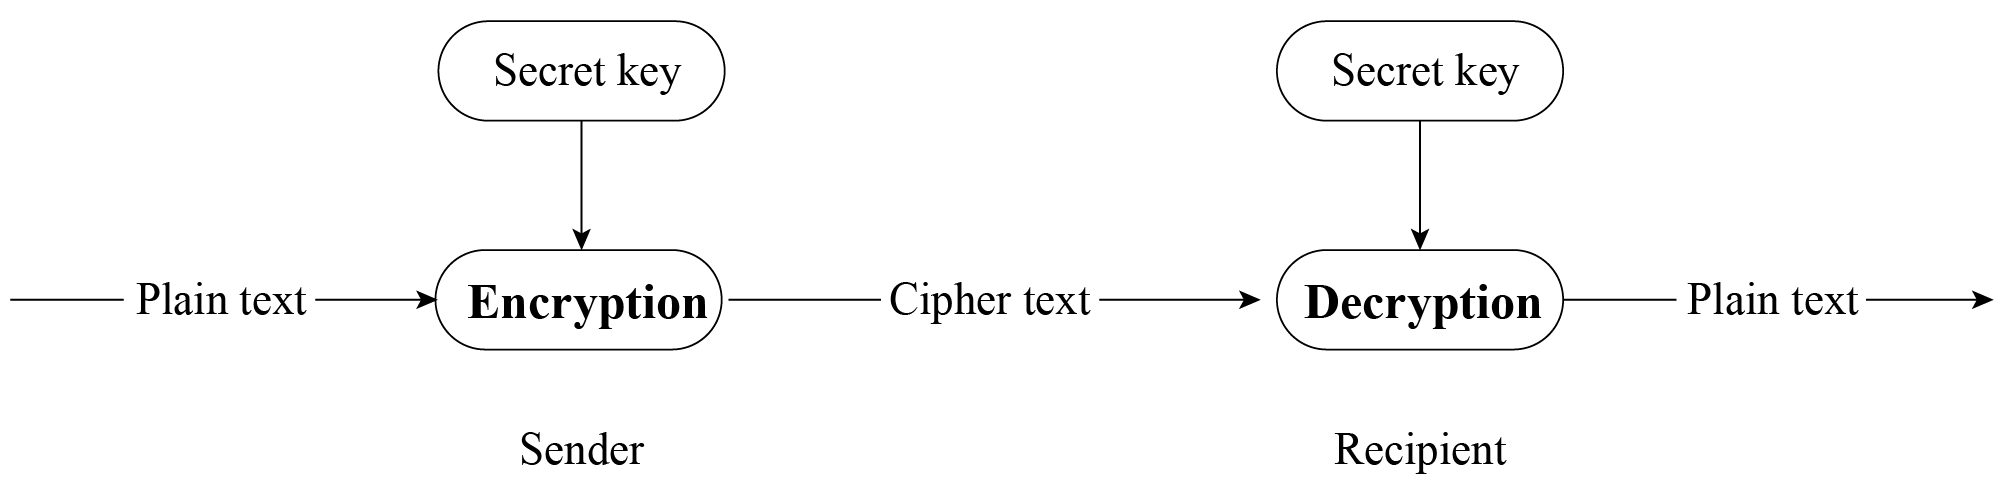
\includegraphics[width=0.8\textwidth]{D8Z/8-11}
    \caption{Process of symmetric encryption}
\end{figure}

In this section, we will introduce the algorithm that is opposite to symmetric encryption, asymmetric encryption. Both parties in asymmetric encryption have a pair of public key and private key. Data is encrypted using the public key, and decrypted using the private key. Because different keys are used for encryption and decryption, this encryption algorithm is called asymmetric encryption. Compared with symmetric encryption, asymmetric encryption is more secure. Because asymmetric encryption is more complex than symmetric encryption, it takes longer time to decrypt, and it is difficult for third parties to directly decipher the data. Because the asymmetric encryption algorithm has high complexity and the private key used for decryption is not transmitted on the network, which can only be obtained by the recipient, this greatly improves data security. Common asymmetric encryption algorithms include RSA, Diffie-Hellman, DSA, etc.

The advantage of asymmetric encryption is its security. User A can keep the private key and transmit the public key to user B through the network. Even if user C obtains the public key, user C cannot decipher the data because user C does not have user A’s private key. In this way, user A and user B can confidently transmit their respective public keys through the network. Remember, the public key is used for encryption, and the private key is used for decryption. Figure 8.12 shows the process of asymmetric encryption.

\begin{figure}[!h]
    \centering
    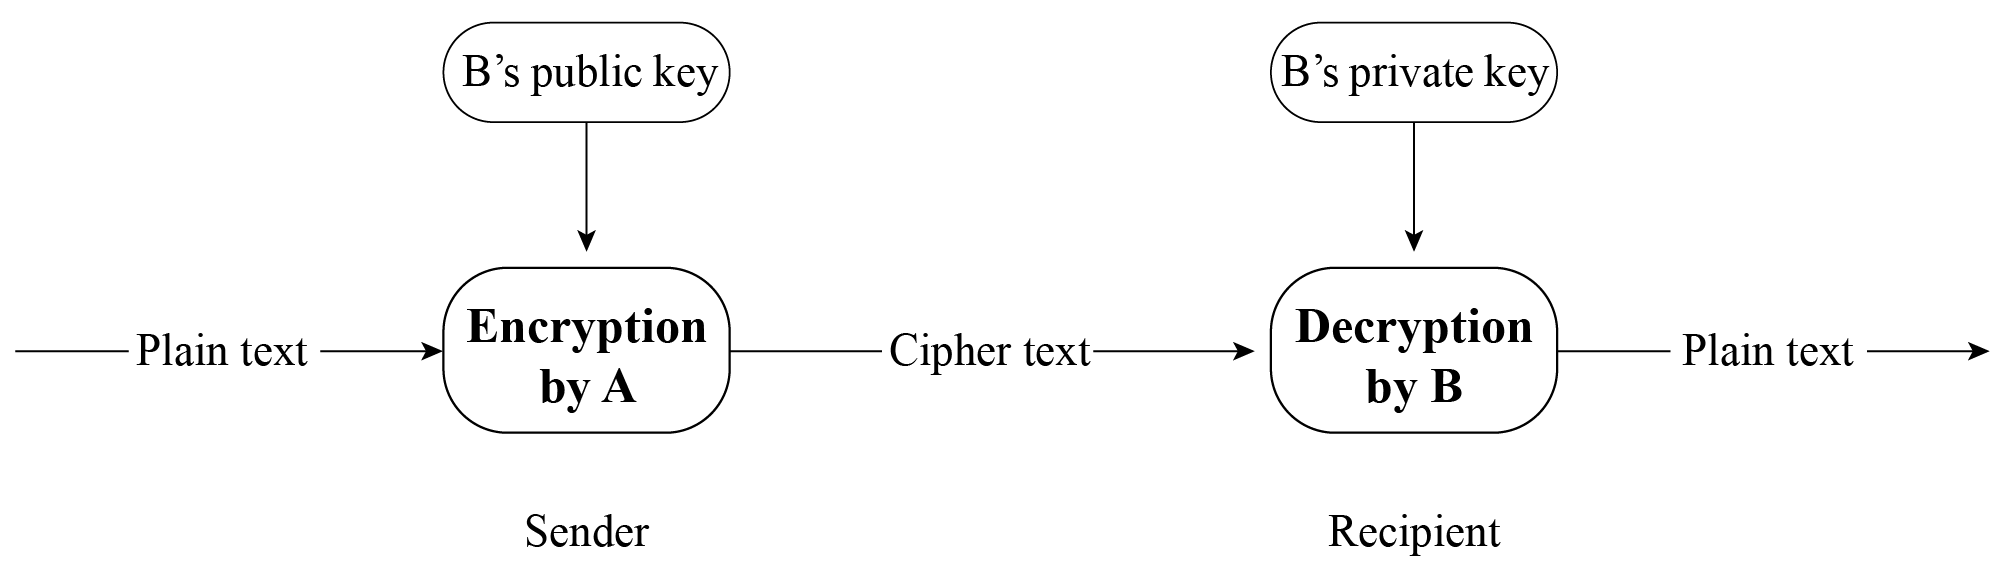
\includegraphics[width=0.8\textwidth]{D8Z/8-12}
    \caption{Process of asymmetric encryption}
\end{figure}

Asymmetric encryption seems very secure, but have you ever thought about this question: what if user C replaces all the public keys sent to user A and user B with its own corresponding private key’s public key? User A does not know whether this public key belongs to user B, so when user A sends data, it will use user C’s public key for encryption. At this time, user C can steal the ciphertext data and decrypt it using the corresponding private key. Therefore, it is crucial to ensure the legitimacy of the public key. In reality, the legitimacy of the public key can be ensured through a Certificate Authority (CA). CA also works based on asymmetric encryption algorithms. With CA, user B will first give its public key and some other information to CA. CA encrypts this data using its private key, and the encrypted data is called user B’s digital certificate. The public key transmitted by user B to user A is the digital certificate encrypted by the CA. After receiving the digital certificate, user A will use the digital certificate published by CA (which contains CA’s public key) to decrypt user B’s digital certificate and obtain user B’s public key.

\subsection{Introduction to Transport Layer Security (TLS)}
TLS is a protocol based on TCP and serves the application layer. Its predecessor is the Secure Socket Layer (SSL) protocol. Through the TLS protocol, the packets of the application layer can be encrypted and delivered to the TCP layer for transmission.

\subsubsection{1. What does TLS do?}
The TLS protocol mainly solves the following three network problems:

\begin{itemize}[leftmargin=1.5em,noitemsep]
    \item Guarantee data confidentiality. All data is transmitted encrypted to ensure protection against unauthorised access or data theft by third parties.
    \item Guarantee data integrity. All data is protected by a verification mechanism, so any tampering will be immediately detected by both parties involved in the communication.
    \item Guarantee the authentication and identity verification of both parties involved in data communication. Certificate authentication can be employed by both parties in the communication to ensure the legitimacy of their identities.
\end{itemize}

\subsubsection{2. How does TLS work?}
The TLS protocol can be divided into two parts. The \textbf{record layer} uses the key negotiated by the client and the server to encrypt and transmit data. The \textbf{handshake layer} negotiates between the client and the server to determine a set of key strings for data transmission encryption. The TLS protocol model is shown in Figure 8.13, where the handshake layer includes four sub-protocols: handshake protocol, change cipher spec protocol, application data protocol, and alert protocol.

\begin{figure}[!h]
    \centering
    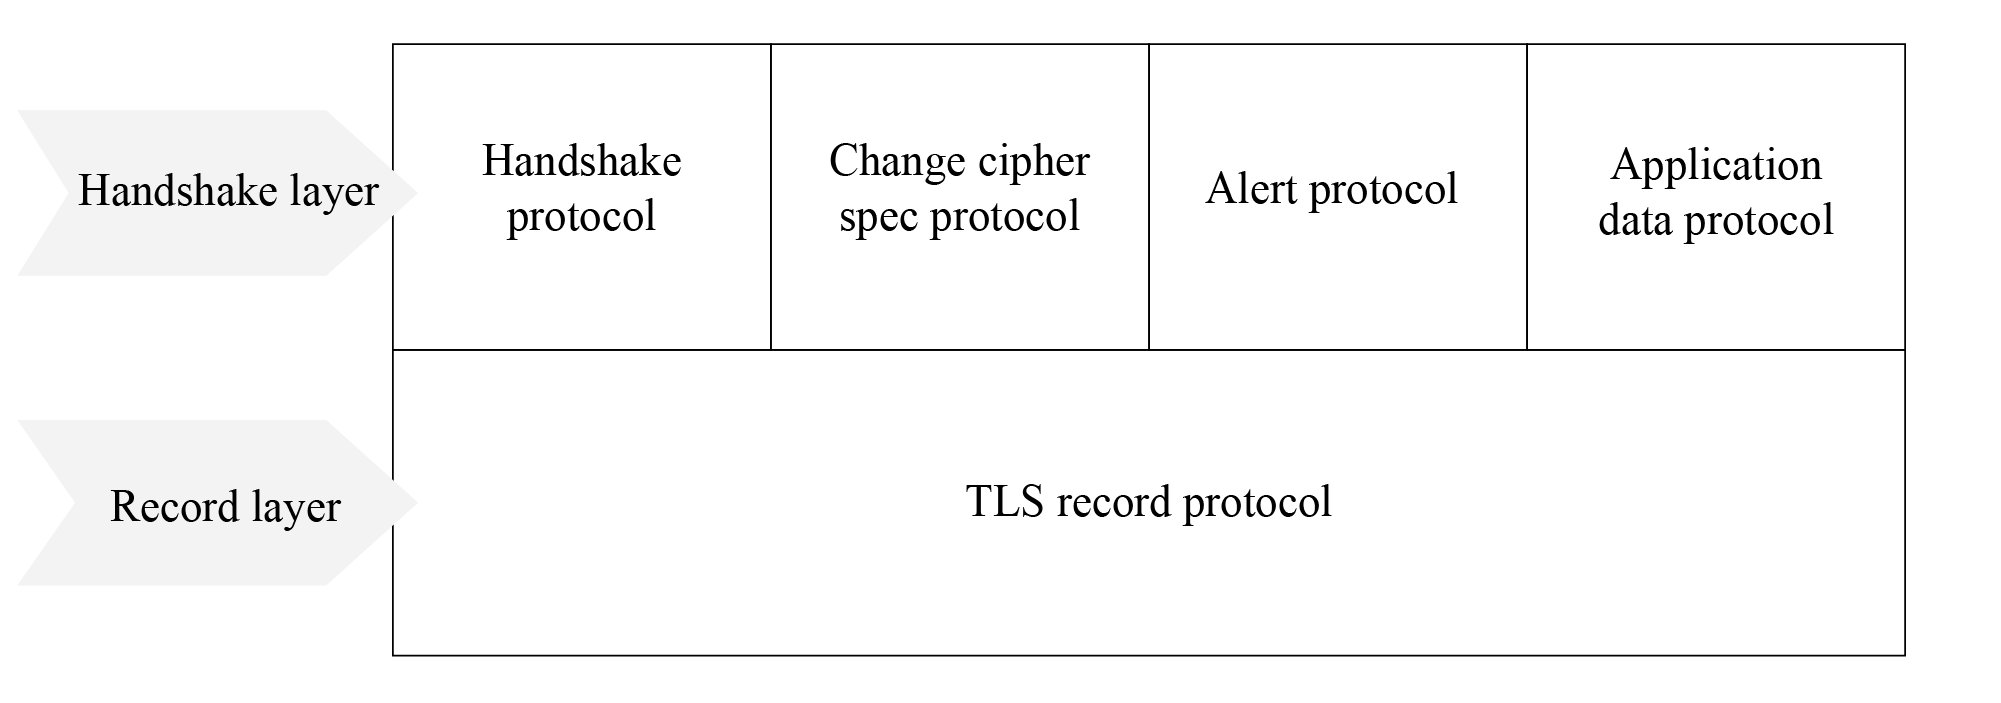
\includegraphics[width=0.7\textwidth]{D8Z/8-13}
    \caption{TLS protocol model}
\end{figure}

Record layer is responsible for all the underlying data exchanged at the transport layer and can encrypt data. Each TLS record begins with a short header, which includes the Content Type (or subprotocol), Protocol Version, and Length fields. The underlying data is segmented (or merged), compressed, added with a message authentication code, encrypted, and then converted into the data part of the TLS record. Figure 8.14 shows the structure of a TLS record packet.

\begin{figure}[!h]
    \centering
    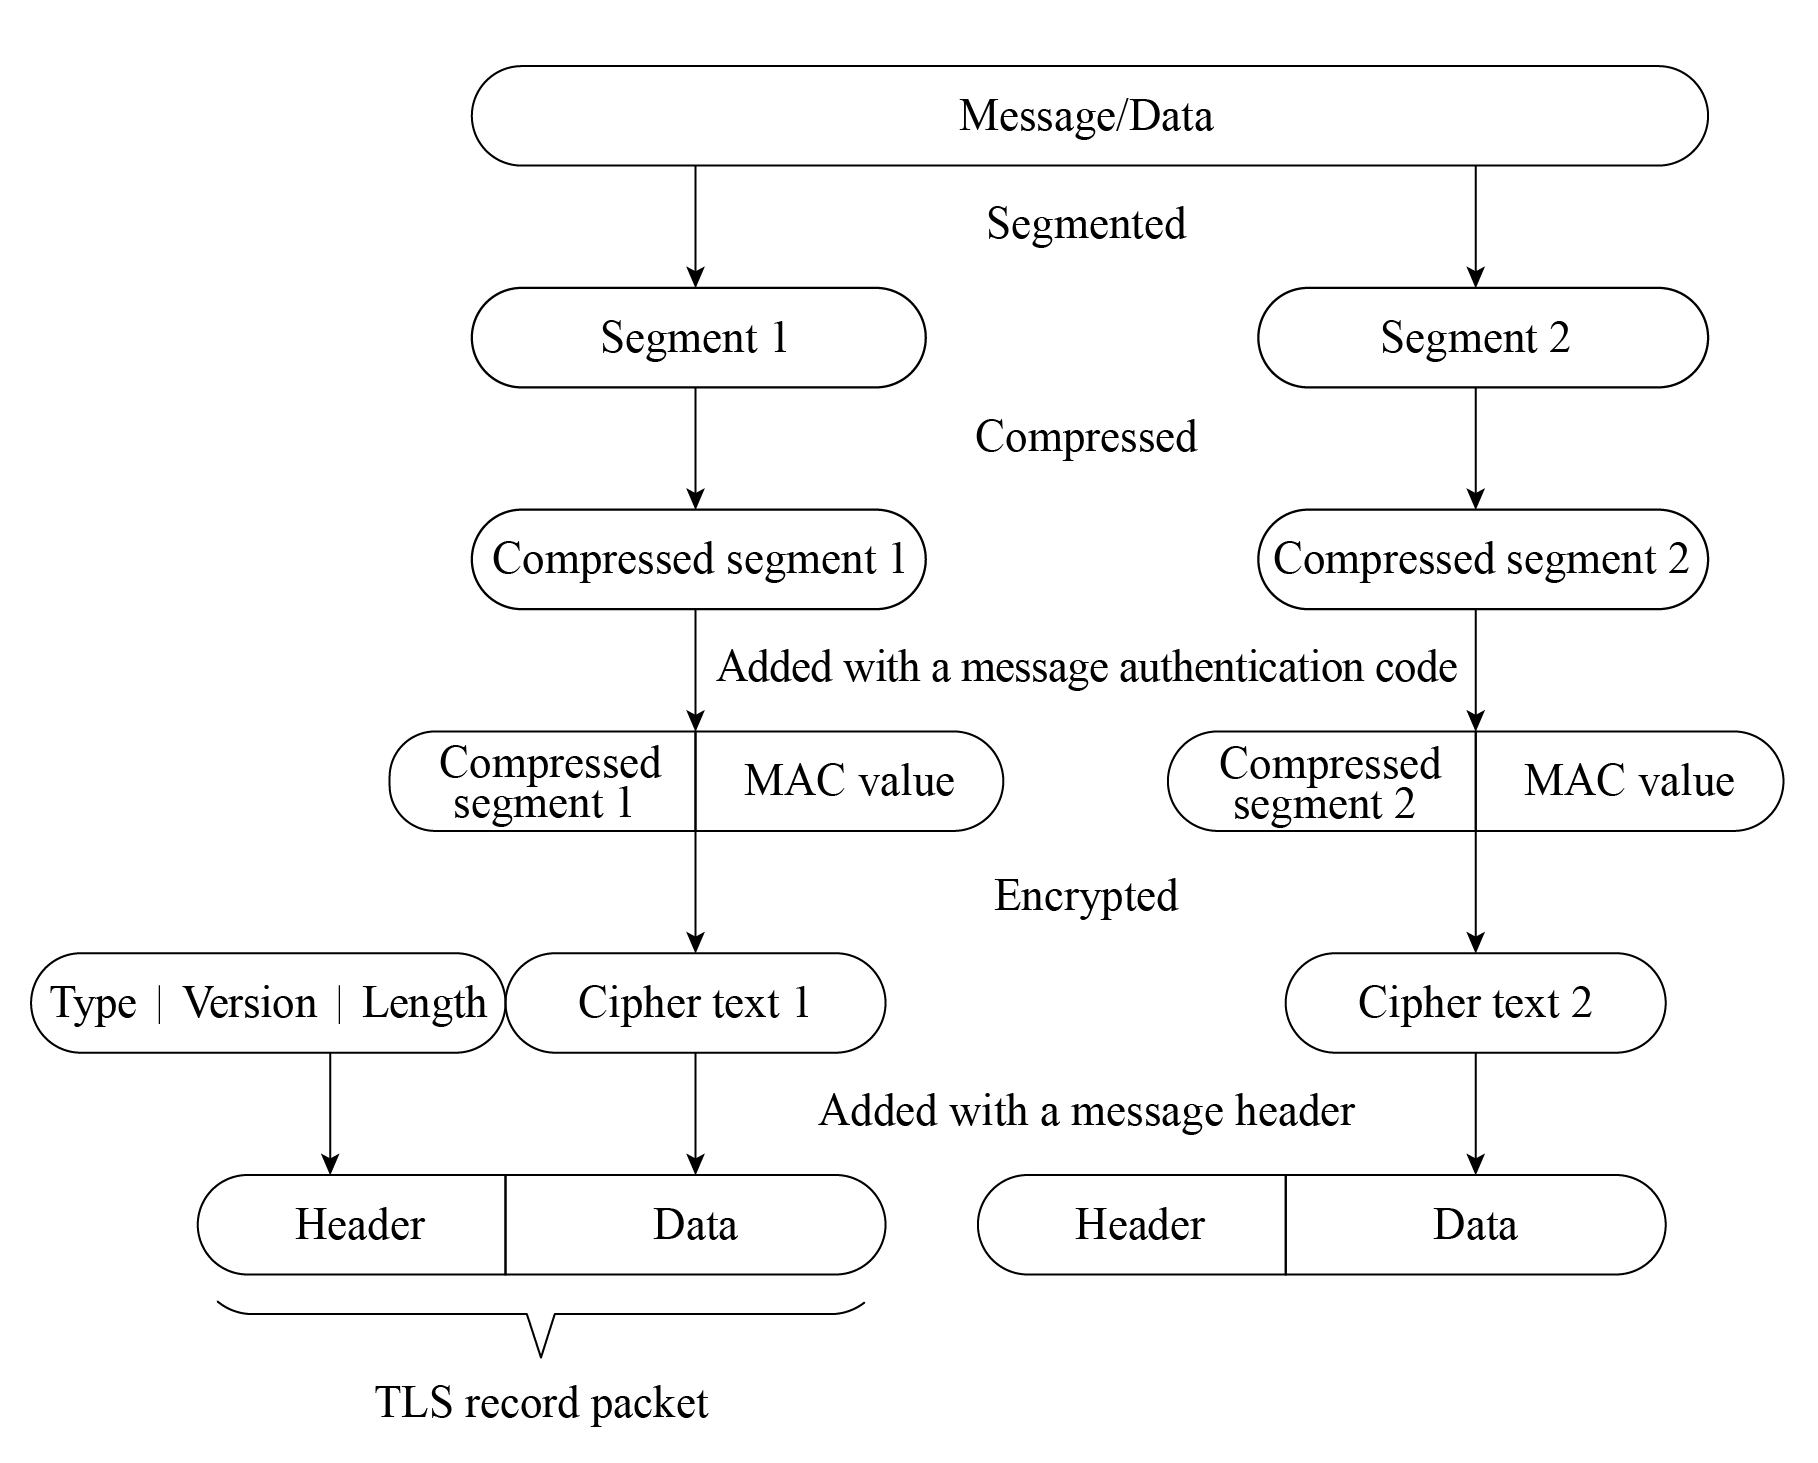
\includegraphics[width=0.66\textwidth]{D8Z/8-14}
    \caption{TLS record packet}
\end{figure}

Handshake layer has four sub-protocols, which are introduced in the list below.

\begin{term}{Handshake protocol}
    Responsible for generating the shared key required for the communication process and performing identity authentication. Note that the handshake protocol does not use cipher suites directly. Instead, it relies on public key cryptography or Diffie-Hellman key exchange to establish secure communication and prevent data from being eavesdropped or intercepted.
\end{term}

\begin{term}{Change cipher spec protocol}
    Responsible for the synchronisation of password switching, and is used after the handshake protocol. During the handshake process, the ‘null’ cipher suite, which means no encryption, is used. After the handshake is completed, the negotiated cipher suite is used for securing the subsequent data transfer.
\end{term}

\begin{term}{Application data protocol}
    Used by the communicating parties for data transmission. The transmission process is carried out through the application data protocol and TLS record protocol of the handshake layer.
\end{term}

\begin{term}{Alert protocol}
    Used to notify the other party when an error occurs, such as an exception during the handshake process, a message authentication code error, or data that cannot be decompressed.
\end{term}

The algorithm used during TLS encryption is introduced in the list below.

\begin{itemize}[noitemsep]
    \item \textbf{Hash function} verifies data integrity. Common encryption algorithms include MD5, SHA, etc.
    \item \textbf{Symmetric encryption} algorithm encrypts the application data. Common encryption algorithms include AES, RC4, DES, etc.
    \item \textbf{Asymmetric encryption} algorithm for identity authentication and key agreement. Common encryption algorithms include RSA, DH, etc.
\end{itemize}

When using TLS, the client and server use asymmetric encryption algorithm to authenticate identity and negotiate the key of symmetric encryption algorithm, and then use symmetric encrypted data and data digest for data communication. Figure 8.15 shows the TLS handshake process.

\begin{figure}[!h]
    \centering
    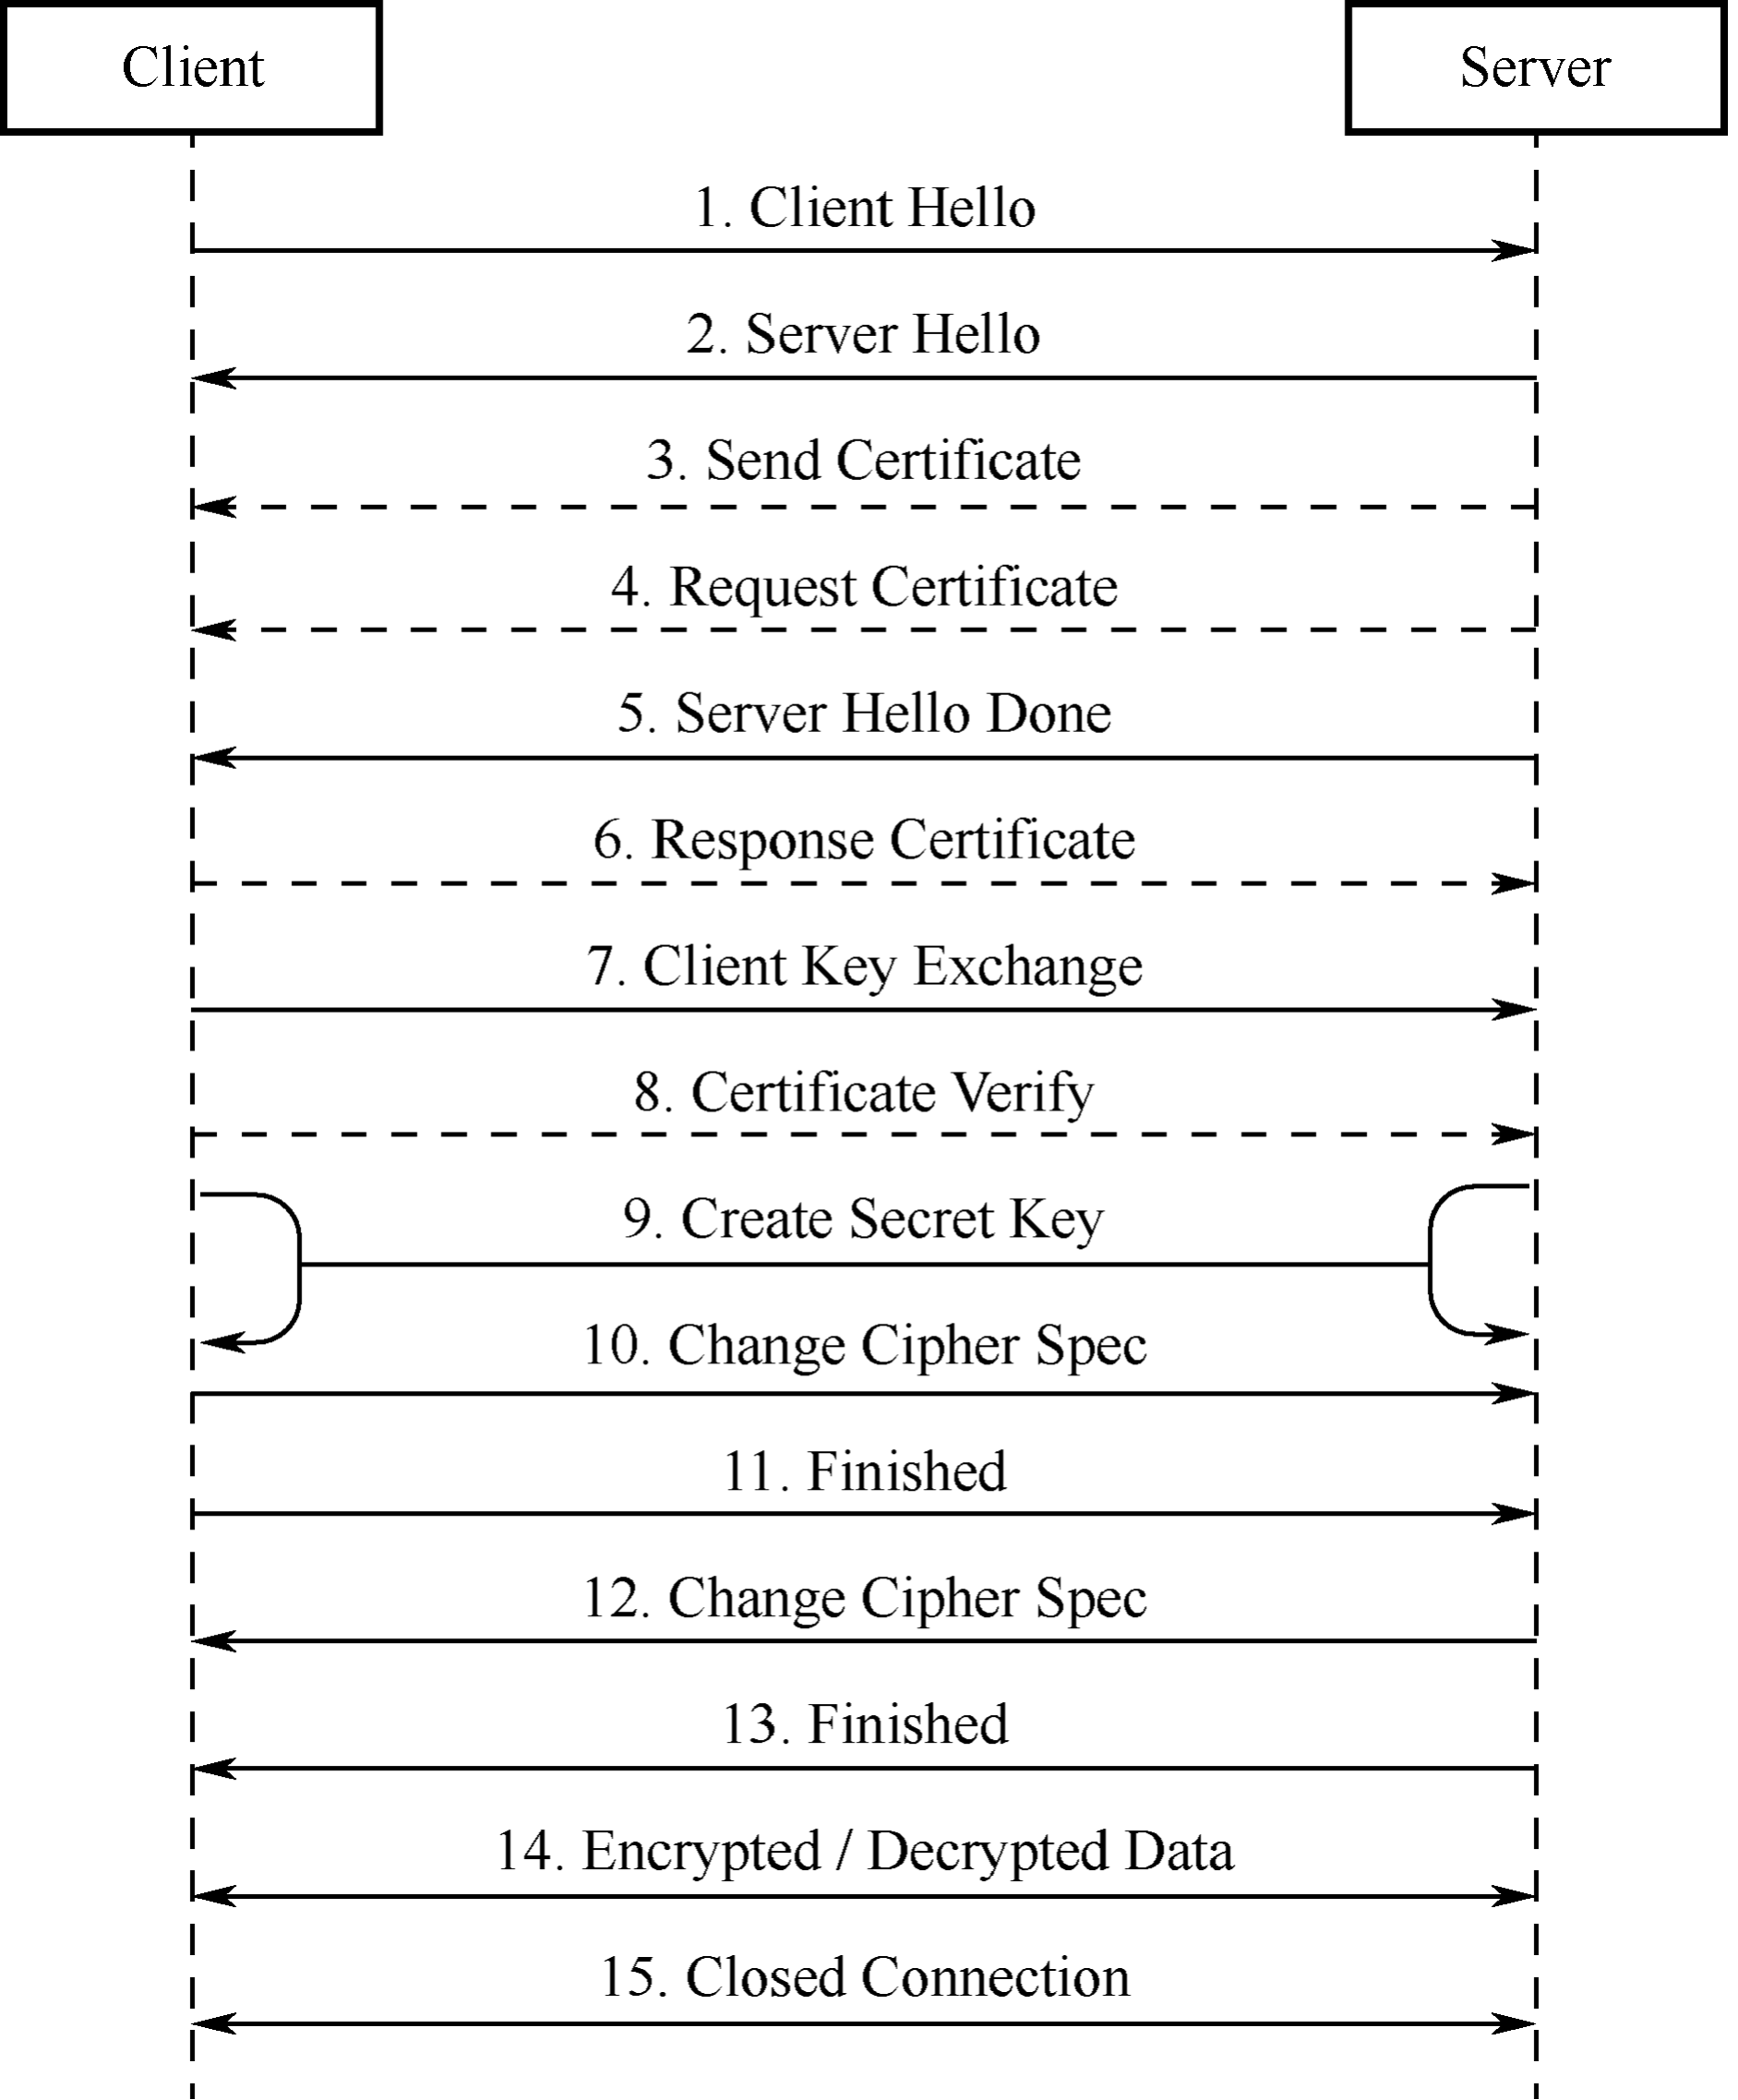
\includegraphics[width=0.5\textwidth]{D8Z/8-15}
    \caption{TLS handshake process}
\end{figure}

\begin{enumerate}[label=(\arabic*)]
    \item Client Hello. The client sends the highest version of the supported TLS protocol and all the cipher suites it supports, which are used to send information such as the random number for generating the session key to the server.
    \item Server Hello. After receiving the Client Hello message sent by the client, the server selects the TLS protocol version and a cipher suite according to the protocol version and cipher suite sent by the client, and returns them to the client.
    \item (Optional) Send Certificate. The server sends its own server-side certificate to the client, which is used by the client to verify the legitimacy of the server.
    \item (Optional) Request Certificate. When the server needs to verify the client’s certificate, the server will send a certificate request message to the client if mutual authentication is selected.
    \item Server Hello Done. The server informs the client that the server has sent all the handshake messages, and the server will wait for the client to send messages.
    \item (Optional) Response Certificate. If mutual authentication is selected, the client will send  its certificate to the server. Then the server will verify the identity of the client.
    \item Client Key Exchange. The client uses the server’s public key to encrypt the client’s public key and key seed before sending them to the server.
    \item (Optional) Certificate Verify. If mutual authentication is selected, the client uses the local private key to generate a digital signature and sends it to the server for authentication through the received client public key.
    \item Create Secret Key. The communicating parties generate the communication key based on information such as the key seed.
    \item Change Cipher Spec. The client notifies the server that the communication method has been switched to encrypted mode.
    \item Finished. The client is ready for encrypted communication.
    \item Change Cipher Spec. The server notifies the client that the communication method has been switched to the encrypted mode.
    \item Finished. Prepare for encrypted communication on the server side.
    \item Encrypted/Decrypted Data. Both parties use the client key to encrypt/decrypt the communication content through a symmetric encryption algorithm.
    \item Closed Connection. After the communication is over, either party sends a message to disconnect the TLS connection.
\end{enumerate}

\subsubsection{3. Creating an HTTP+TLS server with ESP-IDF}
HTTPS, namely HTTP over SSL, encrypts HTTP data through the SSL or TLS protocol. Compared with HTTP, HTTPS can prevent data from being stolen or changed during transmission, thus ensuring data integrity. Section 8.3.2 introduces how to use ESP-IDF to create an HTTP server. In fact, creating an HTTPS server is similar. Call \verb|httpd_ssl_start()| to start the HTTP+TLS service, and call \verb|httpd_register_uri_handler()| to register the corresponding callback function.

\note[Source code]{For the source code of functions \texttt{httpd\_ssl\_start()} and \texttt{httpd\_register\_uri\_hand\newline ler()}, please refer to \href{https://github.com/espressif/book-esp32c3-iot-projects/tree/main/test_case/https_server}{\texttt{book-esp32c3-iot-projects/test\_case/https\_server}}.}

\begin{codebloc}
\begin{tabular}{d}
\vspace{2pt}
\begin{verbatim}
1.  static esperr_t root_get_handler(httpd_req_t *req)
2.  {
3.      httpd_resp_set_type(req, "text/html");
\end{verbatim}
\verb|4.      |\fontsize{9pt}{10pt}\selectfont\verb|httpd_resp_send(req, "<h1>Hello Secure World! </h1>", HTTPD_RESP_USE_STRLEN);|
\footnotesize
\begin{verbatim}
5.      return ESP_OK;
6.  }
7.	
8.  static const httpd_uri_t root = {
9.      .uri       = "/",
\end{verbatim}
\verb|10.     .method = HTTP_GET,|
\end{tabular}
\end{codebloc}

\begin{codebloc}
\begin{tabular}{d}
\vspace{2pt}
\begin{verbatim}
11.     .handler   = root_get_handler
12. };
13.	
14. esp_err_t esp_create_https_server(void)
15. {
16.     httpd_handle_t server = NULL;
17.     ESP_LOGI(TAG, "Starting server");
18.     httpd_ssl_config_t conf = HTTPD_SSL_CONFIG_DEFAULT();
19.     //Configure CA certificate and private key for the server
\end{verbatim}
\verb|20.     |\fontsize{9pt}{10pt}\selectfont\verb|extern const unsigned char cacert_pem_start[] asm("_binary_cacert_pem_start");|

\footnotesize
\verb|21.     |\fontsize{9pt}{10pt}\selectfont\verb|extern const unsigned char cacert_pem_end[] asm("_binary_cacert_pem_end");|
\footnotesize
\begin{verbatim}
22.     conf.cacert_pem = cacert_pem_start;
23.     conf.cacert_len = cacert_pem_end - cacert_pem_start;
\end{verbatim}
\verb|24.     |\fontsize{9pt}{10pt}\selectfont\verb|extern const unsigned char prvtkey_pem_start[] asm("_binary_prvtkey_pem_start");|

\footnotesize
\verb|25.     |\fontsize{9pt}{10pt}\selectfont\verb|extern const unsigned char prvtkey_pem_end[] asm("_binary_prvtkey_pem_end");|
\footnotesize
\begin{verbatim}
26.     conf.prvtkey_pem = prvtkey_pem_start;	
27.     conf.prvtkey_len = prvtkey_pem_end - prvtkey_pem_start;
28.     //Start the HTTP+TLS server
29.     esp_err_t ret = httpd_ssl_start(&server, &conf);
30.     if (ESP_OK ! = ret) {
31.         ESP_LOGI(TAG, "Error starting server!" );
32.         return ESP_FAIL;
33.     }
34.     //Set URI callback function
35.     ESP_LOGI(TAG, "Registering URI handlers");
36.     httpd_register_uri_handler(server, &root);
37.     return ESP_OK;
\end{verbatim}
\verb|38. }|
\end{tabular}
\end{codebloc}

The above code provides an example of how to create an HTTPS server. Before using this code, please manually create a CA certificate and a private key in the \verb|main| directory using the following command:

\begin{codebloc}
\begin{tabular}{d}
\$ \textbf{openssl req -newkey rsa:2048 -nodes -keyout prvtkey.pem -x509 -days 3650 -out cacert.pem -subj "/CN=ESP32 HTTPS server example"}
\end{tabular}
\end{codebloc}

Then modify the \verb|MakeLists.txt| file to compile the certificate into the code.

\begin{codebloc}
\begin{tabular}{d}
\vspace{2pt}
\begin{verbatim}
1.  idf_component_register(SRCS "station_example_main.c"
2.                        INCLUDE_DIRS "."
3.                        EMBED_TXTFILES "cacert.pem"
\end{verbatim}
\verb|4.                        "prvtkey.pem")|
\end{tabular}
\end{codebloc}

In addition, you also need to go to \verb|idf.py menuconfig → Component config → |\\ \verb|ESP HTTPS server|, and configure \verb|CONFIG_ESP_HTTPS_SERVER_ENABLE|.

Enter \verb|https://[your device IP]:443/| in the Chrome browser. The CA certificate on the server side is not issued by a certification authority, thus it is not trusted. Therefore, you will see the screen shown in Figure 8.16.

\begin{figure}[!h]
    \centering
    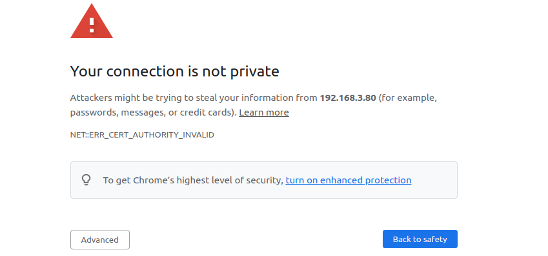
\includegraphics[width=0.65\textwidth,frame]{D8Z/8-16}
    \caption{Interface of untrusted HTTPS connection}
\end{figure}

Users need to click the “Advanced” button to allow this untrusted connection. Figure 8.17 shows the interface of a successful HTTPS connection.

\begin{figure}[!h]
    \centering
    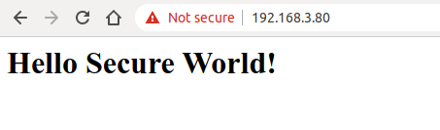
\includegraphics[width=0.6\textwidth,frame]{D8Z/8-17}
    \caption{Interface of successful HTTPS connection}
\end{figure}

Should you encounter a “Header fields are too long for server to interpret” message, just go to \verb|idf.py menuconfig → Component config → HTTP Server → Max HTTP |\\ \verb|Request Header Length|, and increase \verb|HTTPD_MAX_REQ_HDR_LEN|. Figure 8.18 shows the interface where the HTTPS connection fails.

\begin{figure}[!h]
    \centering
    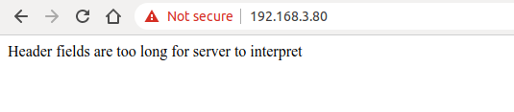
\includegraphics[width=0.7\textwidth,frame]{D8Z/8-18}
    \caption{Interface of HTTPS connection failure}
\end{figure}

\subsection{Introduction to Datagram Transport Layer Security (DTLS)}
DTLS is a UDP-based protocol that serves the application layer. TLS protocol cannot guarantee the security of data transmitted by UDP. Therefore, the DTLS protocol has been extended on the existing TLS protocol architecture to support UDP, and becomes a version of TLS protocol that supports data packet transmission. DTLS 1.0 is based on TLS 1.1, and DTLS 1.2 is based on TLS 1.2. The encryption algorithm, certificate, and encryption process of the DTLS protocol are basically the same as those of the TLS protocol, thus will not be described in this section.

\subsubsection{1. Differences Between DTLS and TLS}
The working principle of the DTLS protocol is basically the same as that of the TLS protocol, except for the following differences:

\begin{itemize}[leftmargin=1.5em]
    \item In the handshake stage, DTLS protocol has added the Cookie mechanism. The DTLS protocol has added a Cookie mechanism in version 1.0, which is used by the server to verify the client, and can avoid DoS attacks. When the client sends the Client Hello message to the server, the server does not directly reply to the Server Hello message to carry out the handshake process. Instead, the server replies the Hello Verify Request message, which carries the Cookie value, to the client. When the client receives the message, it will write the Cookie value into the Client Hello message and resend it to the server. After receiving it, the server checks the local Cookie list to determine whether a handshake is required.
    \item DLTS supports the retransmission mechanism. Since the UDP protocol itself does not support retransmission like the TCP protocol, the DTLS protocol introduces a retransmission mechanism. Taking the above Client Hello message as an example, after the client sends the Client Hello message, the client will start a timer to receive the Hello Verify Request message replied by the server; if the server does not reply within a certain period of time, the client will resend the Client Hello message. Similarly, once a message is sent, the server will activate a timer to monitor for timeouts and determine if the message needs to be resent.
    \item DLTS supports orderly reception. UDP does not guarantee the order of delivered packets. In contrast, DTLS protocol has added a \verb|message_seq| field in the handshake message. The receiver will provide a receiving buffer to receive out-of-order messages (similarly to TCP), and process the messages in order according to the \verb|message_seq| field.
    \item DLTS supports packet size limitation. UDP is a packet-oriented protocol, and TCP is a stream-oriented protocol. TCP supports packet fragmentation and reassembly. However, when a UDP message exceeds the maximum transmission unit (MTU) of the link layer, it may be forcibly fragmented at the IP layer. The receiver then needs to process the fragmented packet based on the IP header and reassemble the original data. If one packet is lost, the entire UDP message will be invalid. Therefore, in DTLS protocol, the handshake messages are segmented on top of UDP. This is done by adding the \verb|fragment_offset| field and \verb|fragment_length| field to the handshake message, which represent the offset of this message relative to the beginning of the message and the length of this message, respectively. 
\end{itemize}

\subsubsection{2. Creating a CoAP+DTLS server with ESP-IDF}
The following example introduces how to create a CoAP+DTLS server. This example is actually the same as the CoAP example introduced in Section 8.3.4, except that two functions are added to support the DTLS protocol. The function \verb|coap_context_set_psk()| is used to set the PSK encryption key in the DTLS protocol, and can also use certificate (PKI) for the DTLS protocol handshake. The \verb|coap_new_endpoint(ctx, &serv_addr, COAP_PRO|\\ \verb|TO_DTLS)| function indicates that the node supports the DTLS protocol.

\note[Source code]{For the complete example code of \texttt{coap\_context\_set\_psk()}, please refer to \href{https://github.com/espressif/book-esp32c3-iot-projects/tree/main/test_case/coap}{\texttt{book-\newline esp32c3-iot-projects/test\_case/coap}}. For instructions on how to use \texttt{PKI}, please see \href{https://github.com/espressif/esp-idf/tree/master/examples/protocols/coap_server}{\texttt{esp-idf/examples/protocols/coap\_server}}.}

\begin{codebloc}
\begin{tabular}{d}
\vspace{2pt}
\begin{verbatim}
1.  static char psk_key[] = "esp32c3_key";
2.  static void esp_create_coaps_server(void)
3.  {
4.      coap_context_t *ctx = NULL;
5.      coap_address_t serv_addr;
6.      coap_resource_t *resource = NULL;
7.      while (1) {
8.          coap_endpoint_t *ep = NULL;
9.          unsigned wait_ms;
10.	
11.         //Create a CoAP server socket
12.         coap_address_init(&serv_addr);
13.         serv_addr.addr.sin6.sin6_family = AF_INET6;
14.         serv_addr.addr.sin6.sin6_port = htons(COAP_DEFAULT_PORT);
15.	
16.         //Create CoAP ctx
17.         ctx = coap_new_context(NULL);
18.         if (!ctx) {
19.             ESP_LOGE(TAG, "coap_new_context() failed");
20.             continue;
21.         }
22.	
23.         //Add PSK encryption key
24.         coap_context_set_psk(ctx, "CoAP",
25.                             (const uint8_t *)psk_key,
26.                             sizeof(psk_key) - 1);
27.	
28.         //Set CoAP node
29.         ep = coap_new_endpoint(ctx, &serv_addr, COAP_PROTO_UDP);
30.         if (!ep) {
31.             ESP_LOGE(TAG, "udp: coap_new_endpoint() failed");
\end{verbatim}
\verb|32.             goto clean_up;|
\end{tabular}
\end{codebloc}

\begin{codebloc}
\begin{tabular}{d}
\vspace{2pt}
\begin{verbatim}
33.         }
34.	
35.         //Add DTLS node and port
36.         if (coap_dtls_is_supported()) {
37.             serv_addr.addr.sin6.sin6_port = htons(COAPS_DEFAULT_PORT);
38.             ep = coap_new_endpoint(ctx, &serv_addr, COAP_PROTO_DTLS);
39.             if (!ep) {
40.                 ESP_LOGE(TAG, "dtls: coap_new_endpoint() failed");
41.                 goto clean_up;
42.             } else {
43.                 ESP_LOGI(TAG, "MbedTLS (D)TLS Server Mode not configured");
44.             }
45.         }
46.	
47.         //Set CoAP resource URI
48.         resource = coap_resource_init(coap_make_str_const("light"), 0);
49.         if (!resource) {
50.             ESP_LOGE(TAG, "coap_resource_init() failed");
51.             goto clean_up;
52.         }
53.	
\end{verbatim}
54. \fontsize{8.5pt}{10pt}\selectfont//Register callback functions for GET and PUT method corresponding to CoAP resource URI
\footnotesize
\begin{verbatim}
55.         coap_register_handler(resource, COAP_REQUEST_GET, esp_coap_get);
56.         coap_register_handler(resource, COAP_REQUEST_PUT, esp_coap_put);
57. 	 
58.         //Set CoAP GET resource visible
59.         coap_resource_set_get_observable(resource, 1);
60.	
61.         //Add resource to CoAP ctx
62.         coap_add_resource(ctx, resource);
63.         wait_ms = COAP_RESOURCE_CHECK_TIME * 1000;
64.         while (1) {
65.             //Wait to receive CoAP data
66.             int result = coap_run_once(ctx, wait_ms);
67.             if (result < 0) {
68.                 break;
69.             } else if (result && (unsigned)result < wait_ms) {
70.                 //Decrease waiting time
71.                 wait_ms -= result;
72.             } else {
73.                 //Reset waiting time
74.                 wait_ms = COAP_RESOURCE_CHECK_TIME * 1000;
75.             }
76.         }
77.     }
78.	clean_up:
\end{verbatim}
\verb|79.     coap_free_context(ctx);|
\end{tabular}
\end{codebloc}

\begin{codebloc}
\begin{tabular}{d}
\verb|80.     coap_cleanup();|

\verb|81. }|
\end{tabular}
\end{codebloc}

\section{Practice: Local Control in Smart Light Project}
The local control component (\verb|esp_local_ctrl|) of ESP-IDF enables you to control Espressif chips via Wi-Fi+HTTPS or Bluetooth LE easily. With this component, you can access application-defined properties, which can be read from or written to through a set of configurable handlers. This section mainly introduces the local control module based on Wi-Fi. Taking the smart light as an example, the local control module can be configured as follows:

\begin{itemize}[noitemsep]
    \item Configure the local device to discover mDNS protocol.
    \item Configure the local HTTPS server and certificate for data communication.
    \item Configure the smart lights.
\end{itemize}

The previous sections have introduced the control of ESP32-C3 via Bluetooth LE. When using Bluetooth LE, the TCP/IP protocol stack is not involved, and local device discovery is not necessary. Bluetooth has its own resource discovery service.

\subsection{Creating a Wi-Fi-based Local Control Server}
The following sample code implements the Wi-Fi-based local control server. The local control is based on HTTP for data communication, and the data is encrypted using the TLS protocol. Additionally, the sample adds the mDNS module for device discovery.

\note[Source code]{For the complete example code, please refer to \href{https://github.com/espressif/book-esp32c3-iot-projects/tree/main/test_case/local_control}{\texttt{book-esp32c3-iot-projects/test\_\newline case/local\_control}}.}

\begin{codebloc}
\begin{tabular}{d}
\vspace{2pt}
\begin{verbatim}
1.  #define PROPERTY_NAME_STATUS "status"
2.  static char light_status[64] = "{\"status\": true}";
3.	
4.  //Property type definition, used with scripts
5.  enum property_types {
6.      PROP_TYPE_TIMESTAMP = 0,
7.      PROP_TYPE_INT32,
8.      PROP_TYPE_BOOLEAN,
9.      PROP_TYPE_STRING,
10. };
11.	
12. //Get attribute value
13. esp_err_t get_property_values(size_t props_count,
14.                               const esp_local_ctrl_prop_t props[],
15.                               esp_local_ctrl_prop_val_t prop_values[],
16.                               void *usr_ctx)
\end{verbatim}
\verb|17. {|
\end{tabular}
\end{codebloc}

\begin{codebloc}
\begin{tabular}{d}
\vspace{2pt}
\begin{verbatim}
18.     int i = 0;
19.     for (i = 0; i < props_count; i ++) {
20.         ESP_LOGI(TAG, "Reading property : %s", props[i].name);
21.         if (!strncmp(PROPERTY_NAME_STATUS,
22.                     props[i].name,
23.                     strlen(props[i].name))) {
24.             prop_values[i].size = strlen(light_status);
25.             prop_values[i].data = &light_status;//prop_values[i].data is 
26.                                   //just a pointer, and cannot be assigned.
27.             break;
28.         }
29.     }
30.     if (i == props_count) {
31.         ESP_LOGE(TAG, "Not found property %s", props[i].name);
32.         return ESP_FAIL;
33.     }
34.     return ESP_OK;
35. }
36.	
37. //Set property value
38. esp_err_t set_property_values(size_t props_count,
39.                               const esp_local_ctrl_prop_t props[],
40.                               const esp_local_ctrl_prop_val_t prop_values[],
41.                               void *usr_ctx)
42. {
43.     int i = 0;
44.     for (i = 0; i < props_count; i ++) {
45.         ESP_LOGI(TAG, "Setting property : %s", props[i].name);
46.         if (!strncmp(PROPERTY_NAME_STATUS,
47.                     props[i].name,
48.                     strlen(props[i].name))) {
49.             memset(light_status, 0, sizeof(light_status));
50.             strncpy(light_status,
51.                     (const char *)prop_values[i].data,
52.                     prop_values[i].size);
53.             if (strstr(light_status, "true")) {
54.                 app_driver_set_state(true); 	//Turn on the smart light
55.             } else {
56.                 app_driver_set_state(false);	//Turn off the smart light
57.             }
58.             break;
59.         }
60.     }
61.     if (i == props_count) {
62.         ESP_LOGE(TAG, "Not found property %s", props[i].name);
63.         return ESP_FAIL;
\end{verbatim}
\verb|64.     }|
\end{tabular}
\end{codebloc}

\begin{codebloc}
\begin{tabular}{d}
\vspace{2pt}
\begin{verbatim}
65.     return ESP_OK;
66. }
67. #define SERVICE_NAME "my_esp_ctrl_device"
68. void esp_local_ctrl_service_start(void)
69. {
70.     //Initialise the HTTPS server-side configuration
71.     httpd_ssl_config_t https_conf = HTTPD_SSL_CONFIG_DEFAULT();
72.     //Load the server certificate
\end{verbatim}
\verb|73.     |\fontsize{9pt}{10pt}\selectfont\verb|extern const unsigned char cacert_pem_start[] asm("_binary_cacert_pem_ start");|

\footnotesize
\verb|74.     |\fontsize{9pt}{10pt}\selectfont\verb|extern const unsigned char cacert_pem_end[]   asm("_binary_cacert_pem_end");|
\footnotesize
\begin{verbatim}
75.     https_conf.cacert_pem = cacert_pem_start;
76.     https_conf.cacert_len = cacert_pem_end - cacert_pem_start;
77.     //Load server-side private key
\end{verbatim}
\verb|78.     |\fontsize{8.9pt}{10pt}\selectfont\verb|extern const unsigned char prvtkey_pem_start[] asm("_binary_prvtkey_pem_ start");|

\footnotesize
\verb|79.     |\fontsize{9pt}{10pt}\selectfont\verb|extern const unsigned char prvtkey_pem_end[] asm("_binary_prvtkey_pem_end");|
\footnotesize
\begin{verbatim}
80.     https_conf.prvtkey_pem = prvtkey_pem_start;
81.     https_conf.prvtkey_len = prvtkey_pem_end - prvtkey_pem_start;
82.     esp_local_ctrl_config_t config = {
83.         .transport = ESP_LOCAL_CTRL_TRANSPORT_HTTPD,
84.         .transport_config = {
85.             .httpd = &https_conf
86.         },
87.         .proto_sec = {
88.             .version = PROTOCOM_SEC0,
89.             .custom_handle = NULL,
90.             .pop = NULL,
91.         },
92.         .handlers = {
93.	
94.             //User-defined processing function
95.             .get_prop_values = get_property_values,
96.             .set_prop_values = set_property_values,
97.             .usr_ctx           = NULL,
98.             .usr_ctx_free_fn = NULL
99.         },
100.
101.        //Set the maximum number of attributes
102.        .max_properties = 10
103.    };
104.
105.    //Initialise local discovery
106.    mdns_init();
107.    mdns_hostname_set(SERVICE_NAME);
108.
109.    //Start the local control service
110.    ESP_ERROR_CHECK(esp_local_ctrl_start(&config));
\end{verbatim}
\verb|111.    |\fontsize{9pt}{10pt}\selectfont\verb|ESP_LOGI(TAG, "esp_local_ctrl service started with name : %s", SERVICE_NAME);|
\end{tabular}
\end{codebloc}

\begin{codebloc}
\begin{tabular}{d}
\vspace{2pt}
\begin{verbatim}
112.    esp_local_ctrl_prop_t status = {
113.        .name        = PROPERTY_NAME_STATUS,
114.        .type        = PROP_TYPE_STRING,
115.        .size        = 0,
116.        .flags       = 0,
117.        .ctx         = NULL,
118.        .ctx_free_fn = NULL
119.    };
120.    //Add attribute value
121.    ESP_ERROR_CHECK(esp_local_ctrl_add_property(&status));
\end{verbatim}
\verb|122.}|
\end{tabular}
\end{codebloc}

The above sample code implements the discovery of a device (domain name: \verb|my_esp_ctrl|\\ \verb|_device.local|) through the local discovery protocol (mDNS), establishes an HTTPS local control connection, and allows the client to set and query attribute values via a registered endpoint.

Users can enable the transmission security protection for local control via the following options:

\begin{itemize}[noitemsep]
    \item PROTOCOM\_SEC0: specifies the end-to-end encryption algorithm used.
    \item PROTOCOM\_SEC1: specifies that data is exchanged as plain text.
    \item PROTOCOM\_SEC\_CUSTOM: customises security requirements.
\end{itemize}

Each attribute must have a unique name (a string), type (e.g., int, bool, or string), flag (e.g., read-only, or readable and writable), and size. If the property value is expected to be of variable length (e.g., if the property value is a string or byte stream), the \verb|size| should be kept at 0. For fixed-length property value data types, such as int, float, etc., setting the size field to the correct value helps \verb|esp_local_ctrl| perform internal checks on parameters received via write requests.

You can process it by matching \verb|props[i].name| with the corresponding property name, and further checking the \verb|flag| and \verb|type| of the property to determine if the property satisfies the corresponding \verb|flag| and \verb|type| requirements.

The default endpoints are shown in Table 8.5.

\begin{table}[h!]
    \renewcommand{\arraystretch}{1}
    \caption{Default endpoints}
    \begin{tabular}{|>{\Centering}m{10em}|>{\Centering}m{15em}|>{\Centering}m{13em}|}
        \hline
        \rowcolor{LightBlue} \textbf{Endpoint name\newline(BLE + GATT Server)}&\textbf{URI (HTTPS Server + mDNS)}&\textbf{Description}\\
        \hline
        esp\_local\_ctrl/version&\url{https://my_esp_ctrl_device.local/esp_local_ctrl/version}&For retrieving version strings\\
        \hline
        esp\_local\_ctrl/control&\url{https://my_esp_ctrl_device.local/esp_local_ctrl/control}&For sending/receiving control messages\\
        \hline
    \end{tabular}
\end{table}

\subsection{Verifying Local Control Functionality using Scripts}
After introducing how to create a local control module, this section will further introduce how to use scripts for verification. Here, we use the official example \verb|esp_local_ctrl| as an example for verification.

\begin{enumerate}[label=\arabic*.,leftmargin=1.5em]
    \item Create a certificate for TLS handshake between the client and the server.

    \begin{enumerate}[leftmargin=0em,label=\alph*.]
        \item Generate a \verb|rootCA| that will be used to sign the server-side certificate, and the client will use it to verify the server-side certificate during the SSL handshake. A passphrase needs to be set to encrypt the generated \verb|rootkey.pem|.

        \begin{codebloc}
        \begin{tabular}{a}
\$ \textbf{openssl req -new -x509 -subj "/CN=root" -days 3650 -sha256 -out rootCA.pem -keyout rootkey.pem}
        \end{tabular}
        \end{codebloc}

        \item Generate a certificate signing request and its private key \verb|prvtkey.pem| for the server.

        \begin{codebloc}
        \begin{tabular}{a}
\$ \textbf{openssl req -newkey rsa:2048 -nodes -keyout prvtkey.pem -days 3650 -out server.csr -subj "/CN=my\_esp\_ctrl\_device.local"}
        \end{tabular}
        \end{codebloc}

        \item Use the previously generated \verb|rootCA| to process the server-side certificate signing request and generate the signing certificate \verb|cacert.pem|. The passphrase set earlier for the encrypted \verb|rootkey.pem| must be entered in this step.

        \begin{codebloc}
        \begin{tabular}{a}
\$ \textbf{openssl x509 -req -in server.csr -CA rootCA.pem -CAkey rootkey.pem -CAcreateserial -out cacert.pem -days 500 -sha256}
        \end{tabular}
        \end{codebloc}

        Among the generated certificates, \verb|cacert.pem| and \verb|prvtkey.pem| are compiled into the server, and \verb|rootkey.pem| is suitable for client-side scripts for server-side verification. The directory of the certificate can be set in the script \verb|esp_local_ctrl.py|.

        \begin{codebloc}
        \begin{tabular}{a}
        \vspace{2pt}
        \fontsize{9pt}{10pt}\selectfont
\begin{verbatim}
1.  def get_transport(sel_transport, service_name, check_hostname):
2.  ...
3.      example_path = os.environ['IDF_PATH'] + '/examples/protocols/esp_local_ctrl'
4.      cert_path = example_path + '/main/certs/rootCA.pem'
\end{verbatim}
\verb|5.  ...|
        \end{tabular}
        \end{codebloc}
    \end{enumerate}

    \item Use the following command to connect to the local control server via script. If \verb|sec_ver| is 0, it means that \verb|PROTOCOM_SEC0| is set on the server.

    \begin{codebloc}
    \begin{tabular}{a}
\$ \textbf{python esp\_local\_ctrl.py --sec\_ver 0}
    \end{tabular}
    \end{codebloc}

    The script will automatically get the property value, i.e.:

    \begin{codebloc}
    \begin{tabular}{a}
    \vspace{2pt}
\begin{verbatim}
Connecting to my_esp_ctrl_device.local

==== Starting Session ====
==== Session Established ====

==== Available Properties ====
S.N. Name             Type       Flags            Value           
\end{verbatim}
\verb|[1] status           STRING                      {"status": true}|
    \end{tabular}
    \end{codebloc}

    \item According to the script prompt, enter the attribute number “1”, and set the attribute value to \verb|{"status": false}|. Then the script will automatically start querying and find that the property value has been changed.

    \begin{codebloc}
    \begin{tabular}{a}
    \vspace{2pt}
\begin{verbatim}
Select properties to set (0 to re-read, 'q' to quit) : 1
Enter value to set for property (status) : {"status": false}
==== Available Properties ====
S.N. Name            Type       Flags            Value           
[1] status           STRING                      {"status": false}  
\end{verbatim}
\verb|Select properties to set (0 to re-read, 'q' to quit) :  |
    \end{tabular}
    \end{codebloc}
\end{enumerate}

\subsection{Creating a Bluetooth-based Local Control Server}
The following sample code creates a Bluetooth-based local control server, which can be used to transmit data. You can refer to the \verb|gatt_server| sample. The following example implements a Bluetooth server. You can compile and flash this example, then use a Bluetooth debugging tool on your smartphone to scan and connect to a Bluetooth device named \verb|ESP32C3-LIGHT|. Once connected, you can access the Bluetooth services provided by the device.

\note[Source code]{For the complete code of the \texttt{gatt\_server} example, please refer to \href{https://github.com/espressif/book-esp32c3-iot-projects/tree/main/test_case/gatt_server}{\texttt{book-esp32c3-\newline iot-projects/test\_case/gatt\_server}}.}

This example provides two Bluetooth services: one for getting the device status (\verb|UUID: FF01|) and another for setting the device status (\verb|UUID: EE01|), as shown in Figure 8.19.

\begin{figure}[!h]
    \centering
    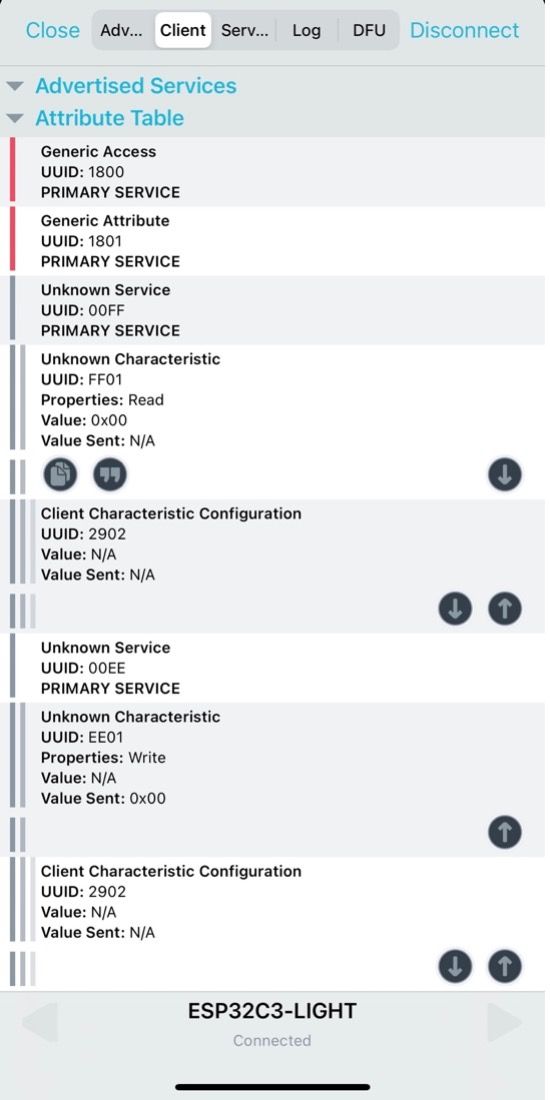
\includegraphics[width=0.37\textwidth]{D8Z/8-19}
    \caption{Bluetooth services in the example}
\end{figure}

The running log is as follows.

\begin{codebloc}
\begin{tabular}{d}
\vspace{2pt}
\begin{verbatim}
I (387) GATTS_DEMO: NVS Flash initialization
I (387) GATTS_DEMO: Application driver initialization
I (397) gpio: GPIO[9]| InputEn: 1| OutputEn: 0| OpenDrain: 0| Pullup: 1|
Pulldown: 0| Intr:0
W (437) BTDM_INIT: esp_bt_controller_mem_release not implemented, return OK
I (437) BTDM_INIT: BT controller compile version [501d88d]
I (437) coexist: coexist rom version 9387209
I (437) phy_init: phy_version 500,985899c,Apr 19 2021,16:05:08
I (617) system_api: Base MAC address is not set
I (617) system_api: read default base MAC address from EFUSE
I (617) BTDM_INIT: Bluetooth MAC: 68:ab:bc:a7:d8:d5
I (637) GATTS_DEMO: REGISTER_APP_EVT, status 0, app_id 0
I (647) GATTS_DEMO: CREATE_SERVICE_EVT, status 0,  service_handle 40
I (647) GATTS_DEMO: SERVICE_START_EVT, status 0, service_handle 40
I (647) GATTS_DEMO: ADD_CHAR_EVT, status 0,  attr_handle 42, service_handle 40
I (657) GATTS_DEMO: ADD_DESCR_EVT, status 0, attr_handle 43, service_handle 40
\end{verbatim}
\verb|I (667) GATTS_DEMO: REGISTER_APP_EVT, status 0, app_id 1|
\end{tabular}
\end{codebloc}

\begin{codebloc}
\begin{tabular}{d}
\vspace{2pt}
\begin{verbatim}
I (677) GATTS_DEMO: CREATE_SERVICE_EVT, status 0,  service_handle 44
I (677) GATTS_DEMO: SERVICE_START_EVT, status 0, service_handle 44
I (687) GATTS_DEMO: ADD_CHAR_EVT, status 0,  attr_handle 46, service_handle 44
I (697) GATTS_DEMO: ADD_DESCR_EVT, status 0, attr_handle 47, service_handle 44
I (6687) GATTS_DEMO: ESP_GATTS_CONNECT_EVT, conn_id 0, remote 4a:13:d8:ca:b3:cf:
I (6687) GATTS_DEMO: CONNECT_EVT, conn_id 0, remote 4a:13:d8:ca:b3:cf:
I (6987) GATTS_DEMO: ESP_GATTS_MTU_EVT, MTU 500
I (6987) GATTS_DEMO: ESP_GATTS_MTU_EVT, MTU 500
I (7347) GATTS_DEMO: update connection params status = 0, min_int = 16, max_int
= 32,conn_int = 24,latency = 0, timeout = 400
I (15117) GATTS_DEMO: GATT_READ_EVT, conn_id 0, trans_id 3, handle 42
I (23037) GATTS_DEMO: GATT_WRITE_EVT, conn_id 0, trans_id 4, handle 46
I (23037) GATTS_DEMO: GATT_WRITE_EVT, value len 1, value :
I (23037) GATTS_DEMO: 00 
I (23037) app_driver: Light OFF
I (30987) GATTS_DEMO: GATT_WRITE_EVT, conn_id 0, trans_id 5, handle 46
I (30987) GATTS_DEMO: GATT_WRITE_EVT, value len 1, value :
I (30987) GATTS_DEMO: 01 
\end{verbatim}
\verb|I (30987) app_driver: Light ON|
\end{tabular}
\end{codebloc}

\section{Summary}
In this chapter, we first presented an overview of the framework model, applicable conditions, and application scenarios of local control. We also compared it to remote control, enabling you to assess the suitability of local control functionality based on your unique project requirements. Local discovery plays a pivotal role in local control as it governs the ability of smartphones to search for devices within the LAN. This allows smartphones to retrieve device characteristics and facilitates subsequent control of the identified devices. Therefore, we also delved into the operational mode of the local discovery protocols, specifically in terms of the principle layer. We also conducted a comparative analysis of the characteristics of the two modes: broadcast and multicast, shedding light on their similarities and differences. The most commonly used local discovery protocol is mDNS, which provides you with the flexibility to implement local discovery functionality in your IoT projects. You can also leverage the resource discovery technology inherent in the Bluetooth protocol directly when utilising Bluetooth for control purposes.

Then we introduced the most critical data communication protocols and corresponding data encryption algorithms in local control. The fundamental protocols for data communication in local control are TCP and UDP . While you can directly utilise these protocols for local control, it is generally not recommended due to certain limitations. TCP and UDP are classified as transport layer protocols and do not inherently carry application format data, in contrast to protocols like HTTP and CoAP, which incorporate an application layer on top of the transport layer. Furthermore, it’s important to note that transport layer protocols such as TCP and UDP do not support direct encryption of data using protocols like TLS or DTLS. Therefore, relying solely on the transport layer protocol for data transmission may not guarantee the security of the transmitted data. Hence, it is recommended that you utilise protocols such as HTTP with TLS or CoAP with DTLS for data communication in local control scenarios. 

Finally, we introduced how to implement the complete local control function based on the \verb|esp_local_ctrl| component in ESP-IDF. \verb|esp_local_ctrl| supports local control based on Wi-Fi and Bluetooth, with data communication protocols that include HTTPS for Wi-Fi and Bluetooth protocols for Bluetooth. You can get started with local control development with \verb|esp_local_ctrl| component. Additionally, the \verb|esp_local_ctrl| component does not support local network device discovery functionality. You need to implement device discovery functionality using the mDNS module. The \verb|esp_local_ctrl| component is widely used in ESP-IDF, and you can find provisioning and local communication features in the \verb|wifi_provisioning| component for network configuration and local communication.

Of course, there are various protocols and implementation methods for local control. If the \verb|esp_local_ctrl| component does not meet your requirements, you can follow the example codes in sections 8.2, 8.3, and 8.4 to build your own local control framework.

\end{document}